 \documentclass[]{article}
\usepackage{graphicx,array,tabu,subcaption,float,glossaries,url,amsmath}
\usepackage{geometry}
\geometry{a4paper,portrait, margin=1in}
\usepackage[T1]{fontenc}
\newcommand\numberthis{\addtocounter{equation}{1}\tag{\theequation}}
\graphicspath{{/home/shenoy/Documents/Nikhil/research/RADICAL-research/slade_paper/img/}}

\begin{document}
\title{Performance Summary of Ensemble-MD Patterns}
\author{Nikhil Shenoy}
\date{\today}
\maketitle

\abstract{Modern software, no matter its application, always incorporates performance as a design factor. Characterizations of the performance of such software informs the user about how the system will behave when given certain inputs, which the user can then leverage to create efficient applications. Accurate characterizations of performance can augment the speed of development, as the developer can easily assess which parts of the system are bottlenecks and fix them directly. Without these efficient characterizations, the software becomes less attractive to the user because its behavior is not well-defined. Such attributes are seriously considered when designing software for scientific computing, as many simulations in areas such as molecular dynamics, bio-molecular dynamics, and genomics rely on consistent performance to process the ever-increasing amount of data. In this article, we discuss the EnsembleMD-Toolkit (EnMD Toolkit) and benchmark the efficiency of two standard Patterns using a sample workload. We also compare the performance of RADICAL-Pilot (RP) with that of RADICAL-Pilot extended with Apache Hadoop YARN (RP-YARN) using a clustering example. We assume that the reader has a basic familiarity with the softwares, and we will only define parameters relevant to the performed experiments.}

\section{Introduction}

	\subsection{Motivations}
		Traditional distributed systems utilize batch queueing systems in order to schedule jobs to a high performance machine's resources. In such systems, scripts are written to execute several different tasks sequentially, and a scheduler assigns the tasks to the resources it requires. The problem with this approach is that since a task will most likely require only a fraction of the available resources, the remaining resources will stay idle. Leaving cores unutilized severely limits the efficiency and throughput of the system and must be avoided. Additionally, the total waiting time in the queue for a simulation can scale quickly in the number of component tasks, which can significantly increase the time to completion. These problems burden the user who, in many cases, is attempting to run computation-heavy scientific simulations \cite{vishal_shah_paper}.

		To alleviate this problem, the concept of Pilot-Jobs was introduced. In a pilot scheme, information about each task of a multi-task simulation is associated with the pilot, and only the pilot is placed into the scheduling queue. Once the pilot is scheduled to a machine, it can then request and execute multiple tasks on its assigned resources. By placing only the pilot into the scheduling queue, the user circumvents the scheduler and obviates the time necessary to request and assign resources for the total number of tasks. This can result in a decreased time-to-completion for each task, and high throughput of the number of tasks \cite{rp_paper}.

		The RADICAL-Cybertools group implemented RADICAL-Pilot API as an instance of a Pilot Job system, and it can be used as a standalone software package. However, the group has also used it as a platform to develop software for different scientific use cases. The Replica Exchange, ExTASY, and EnsembleMD Toolkit are all examples of packages that utilize RADICAL-Pilot in the backend to execute simulations. Using the pilot paradigm as a platform for high performance science provides developers with a unique type of abstraction; all of the information regarding scheduling, queueing, resource management, and communication has been completely abstracted from the user. The EnsembleMD-Toolkit, an API designed for large scale molecular dynamics simulations, is a prime example of this, as it utilizes RADICAL-Pilot to implement simulations that are popular within the molecular dynamics community. Making the EnsembleMD Toolkit a client to RADICAL-Pilot in the architecture allows the client scientist to focus entirely on the science at hand rather than the intricacies of distributed systems, since they are all hidden from the user. From the perspective of an EnsembleMD developer, generating new application patterns and kernels for the Toolkit becomes much easier since the mechanism for job submission and management is decoupled from the logic of the use cases. Thus, both clients and developers of the EnsembleMD software can meet the demands of expedient execution of simulations as well as extensibility and continued development of the software.

		However, constructing this architecture is not enough. If a client is looking for optimal performance out of a system, he must be aware of all the different components and their behaviour under varied conditions before determining whether the system is useful to him. For this reason it is important to construct accurate performance profiles for software like EnsembleMD, as its utility depends on its ability to perform well at large scales. Factors that must be considered when designing such a profile include the costs of communication between nodes and other entities, the volume of data that can be transferred, the overall time-to-completion, and the overheads incurred by each component. Analyzing these components allows a developer to identify bottlenecks in the system and work to fix them in order to make the software more attractive to the user.

		Aside from the EnsembleMD toolkit, the RADICAL-Pilot API offers an improvement in efficiency for HPC tasks. While it is not designed to handle data-intensive tasks, Apache Hadoop and YARN are able to work on problems involving large amounts of data. YARN in particular plays the roles of resource manager and scheduler in this context, and contributes the main functionality for wrestling with large volumes of data \cite{apache_hadoop_yarn}. RADICAL-Pilot has been extended with YARN in order present an iterface which has performs well on HPC and data-intensive tasks. This extension gives birth to the RADICAL-Pilot-YARN package, which contains functionality to operate on HPC and data-intensive tasks. In this paper, we will examine the performance of RADICAL-Pilot-YARN in comparison to RADICAL-Pilot by itself using a simulation of a simple clustering algorithm. We will also examine the performance of the EnsembleMD Toolkit in the hope of constructing a comprehensive performance profile by examining the various components of the EnsembleMD Toolkit under a set workload.

	\subsection{Ensemble-MD Toolkit} 
		In this article, we present the EnsembleMD Toolkit (EnMD) as one of the complex applications built on top of the RADICAL-Pilot architecture, and provide a brief overview of the software here. The execution flow of the Toolkit is centered around three main components; the Application Pattern, the Execution Context, and the Kernel Plugin. 

		% Architecture Diagram?

		The first component that the user interacts with, the Application Pattern, is a general template for executing tasks. These patterns present the user with high-level descriptions of control flow which are task-independent. The user need only choose a pattern and provide it with the details necessary for the simulation, and the API takes care of the rest. By doing this, the details of executing the simulation are abstracted from the user, providing an interface that makes translating biological experiments into computer simulations very simple. For example, the Pipeline Application Pattern can run a collection of tasks sequentially as a series of steps. In this scheme, the pattern will wait for each step to finish before moving on to the next step. The pattern also allows for several instances of a given pipeline, as shown in Figure 1, if redundancy is required. Other available patterns include Simulation-Analysis and the Replica Exchange \cite{enmd_paper}, \cite{repex_paper}.

		\begin{figure}[H]
			\centering
			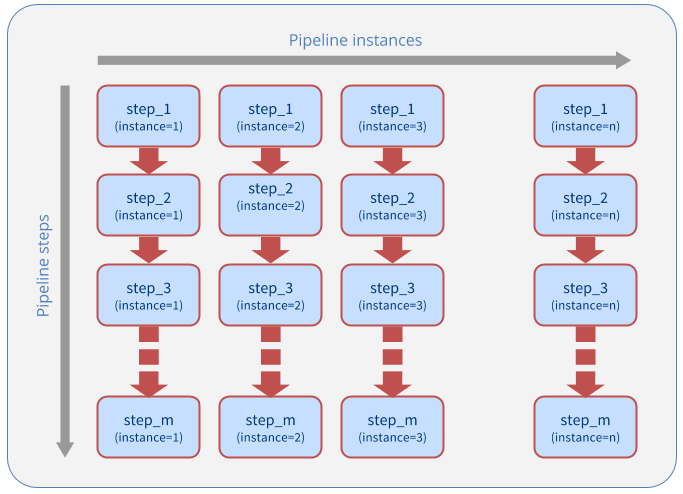
\includegraphics[width=7cm,height=5cm]{pipeline_pattern}
			\caption{Block Diagram of the Pipeline Pattern \cite{pipeline_pattern}}
			\label{fig:pipeline_block_diagram}
		\end{figure}

		The Execution Context represents the distributed computing resource that the simulation is running on. It contains the infrastructure needed to interface with the machine itself, and is the agent that allows the Toolkit to adapt to and include a variety of resources. Its main functions are to allocate and deallocate the resource, as well as run an execution pattern on the resource. Aside from specifying which resource to use, the user does not interact with this component directly as it is meant to be behind the wall of abstraction. 

		Finally, the Kernel Plugin represents the scientific tool to be used. This can be anything from molecular dynamics executables such as Amber to simple tasks such as counting the number of characters in a file. The Toolkit provides a list of built-in kernels, but provides a mechanism for users to add their own. The Kernel Plugin abstracts aspects of the tools that are specific to a particular resource and presents a uniform interface with the user can define tasks \cite{enmd_paper}.

		Using this three basic components, EnsembleMD is able to characterize biological phenomena and run simulations specific to those phenomena. However, recent efforts in the development of the Toolkit have led to applications in astronomy, specifically in monitoring the \textit{movement of galaxies}. The abstractions for biological phenomena provided by the Toolkit are thus shown to not only be effective for those types of simulations, but can also be extended to fit other science applications as well.

	\subsection{RADICAL-Pilot and RADICAL-Pilot-YARN}
		RADICAL-Pilot is a Python API developed by the RADICAL-Cybertools group that aids developers in submitting and running batches of tasks on high performance machines. The API achieves this through a container called a Pilot; this container is assigned the information associated with each task in the batch, such as the location of input data and what simulation to run, and is then placed in the queue of an HPC machine. Once the scheduler on the HPC machine schedules the Pilot onto a resource, the Pilot will then start its own Agent to begin carrying out the batch of tasks. It aggregates all the necessary resources, and then pulls additional information about each task from MongoDB. The Agent is responsible for carrying out the execution for each task and making sure that the output is sent back to the user.

		\begin{figure}[H]
			\centering
			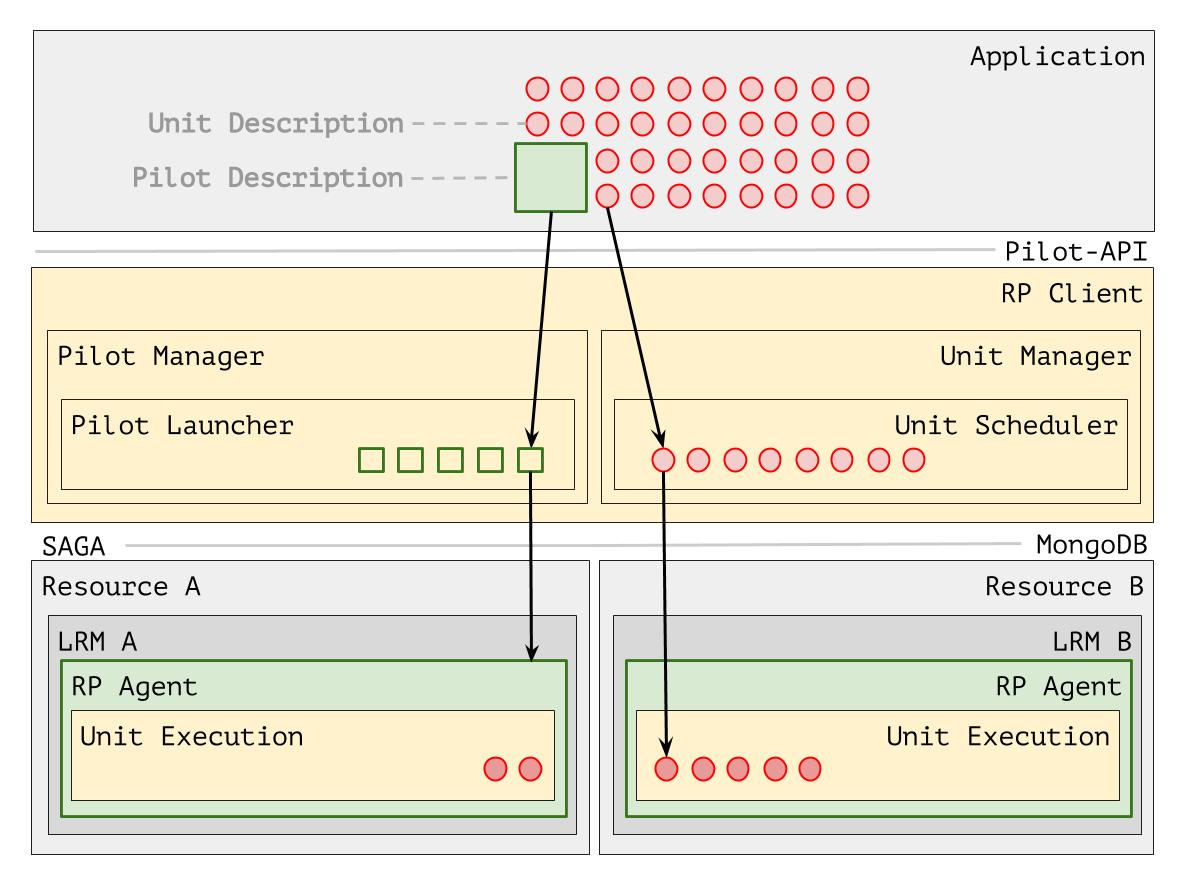
\includegraphics[width=7cm,height=5cm]{rp_arch}
			\caption{The RADICAL-Pilot Architecture \cite{rp_arch}}
			\label{fig:rp_architecture}
		\end{figure}

		This method of scheduling tasks provides many advantages, one of which is circumventing the scheduler. In current submission scenarios, each task must occupy a place in the scheduling queue and must individually wait for the required resources to become available before executing. This greatly increases the total time spent in the queue for the collection of tasks, which also increases the time to completion. However, Pilots allow users to avoid this time penalty by taking advantage of late binding and sending only the Pilot through the scheduler, reducing the wait time to that of a single task. Once the Pilot is finally scheduled, the user can then employ the various execution styles provided by the API based on the nature of their application. For example, if the batch is split into two types of tasks where one must occur before the other, the API provides functionality to schedule and execute such chained tasks. This, and the other options provided by RADICAL-Pilot, presents the user with a simple but powerful interface for task execution that outstrips current methods. By permitting any executable to be associated with a task in a Pilot, the RADICAL-Pilot API is flexible enough to handle a variety of HPC tasks, making it ideal for users who regularly work on the order of thousands of simulations.

		As previously mentioned, RADICAL-Pilot's strength lies in managing high performance computing tasks. Apache Hadoop and YARN, on the other hand, are designed for simulations requiring large volumes and types of data. To provide RADICAL-Pilot with the capability to work on both types of tasks, it has been extended with various components from YARN, which we detail here. The extensions have been implemented at the level of RADICAL-Pilot's Agent, the entity responsible for coordinating execution on the remote machine. The Local Resource Manager now retrieves new environment variables that detail the number of cores to be used on each node and the assignment of nodes, among other parameters. It then passes this information on to the newly started Hadoop and YARN demons, which examine and record the current state of the cluster.

		\begin{figure}[H]
			\centering
			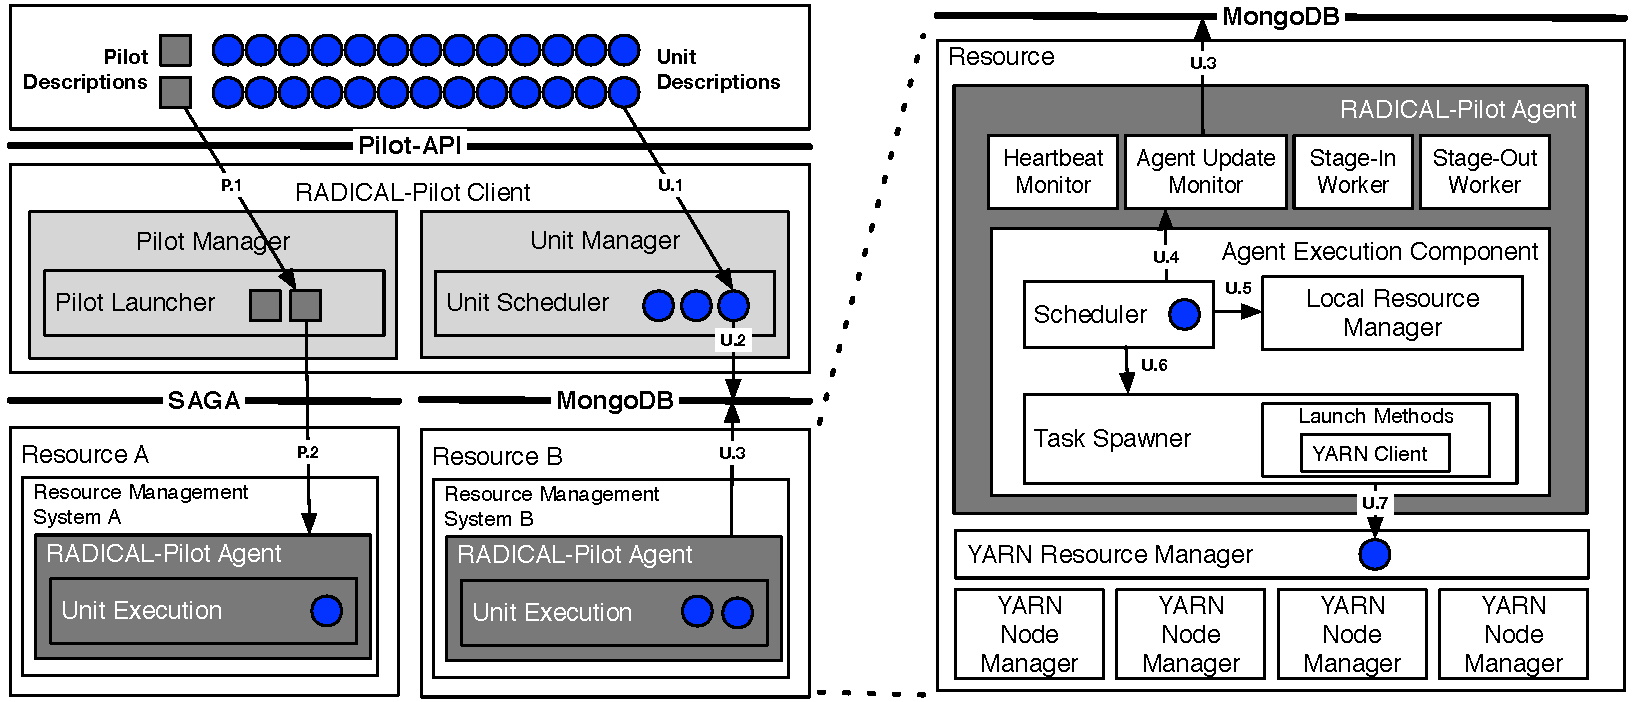
\includegraphics[scale=.42]{rp-architecture-yarn.pdf}
			\caption{The RADICAL-Pilot-YARN Architecture. As seen in \cite{hadoop_paper}.}
			\label{fig:rp_yarn_arch}
		\end{figure}

		The RADICAL-Pilot scheduler has also been updated to include information about the current state of the cluster, including updates on the total memory available and the total number of cores in use. The scheduler then uses this state information to schedule the next task appropriately. Finally, the Application Manager, which handles the resource allocations, works with the YARN Resource Manager in order to coordinate the execution of tasks. RADICAL-Pilot provisions a Compute Unit with a Description that contains the resource requirements, and then requests that YARN create a container for it. By placing the Compute Unit within the YARN container, the YARN scheduler can then easily assign the container the optimal resources for execution \cite{hadoop_paper}. 

		\begin{figure}[H]
			\centering
			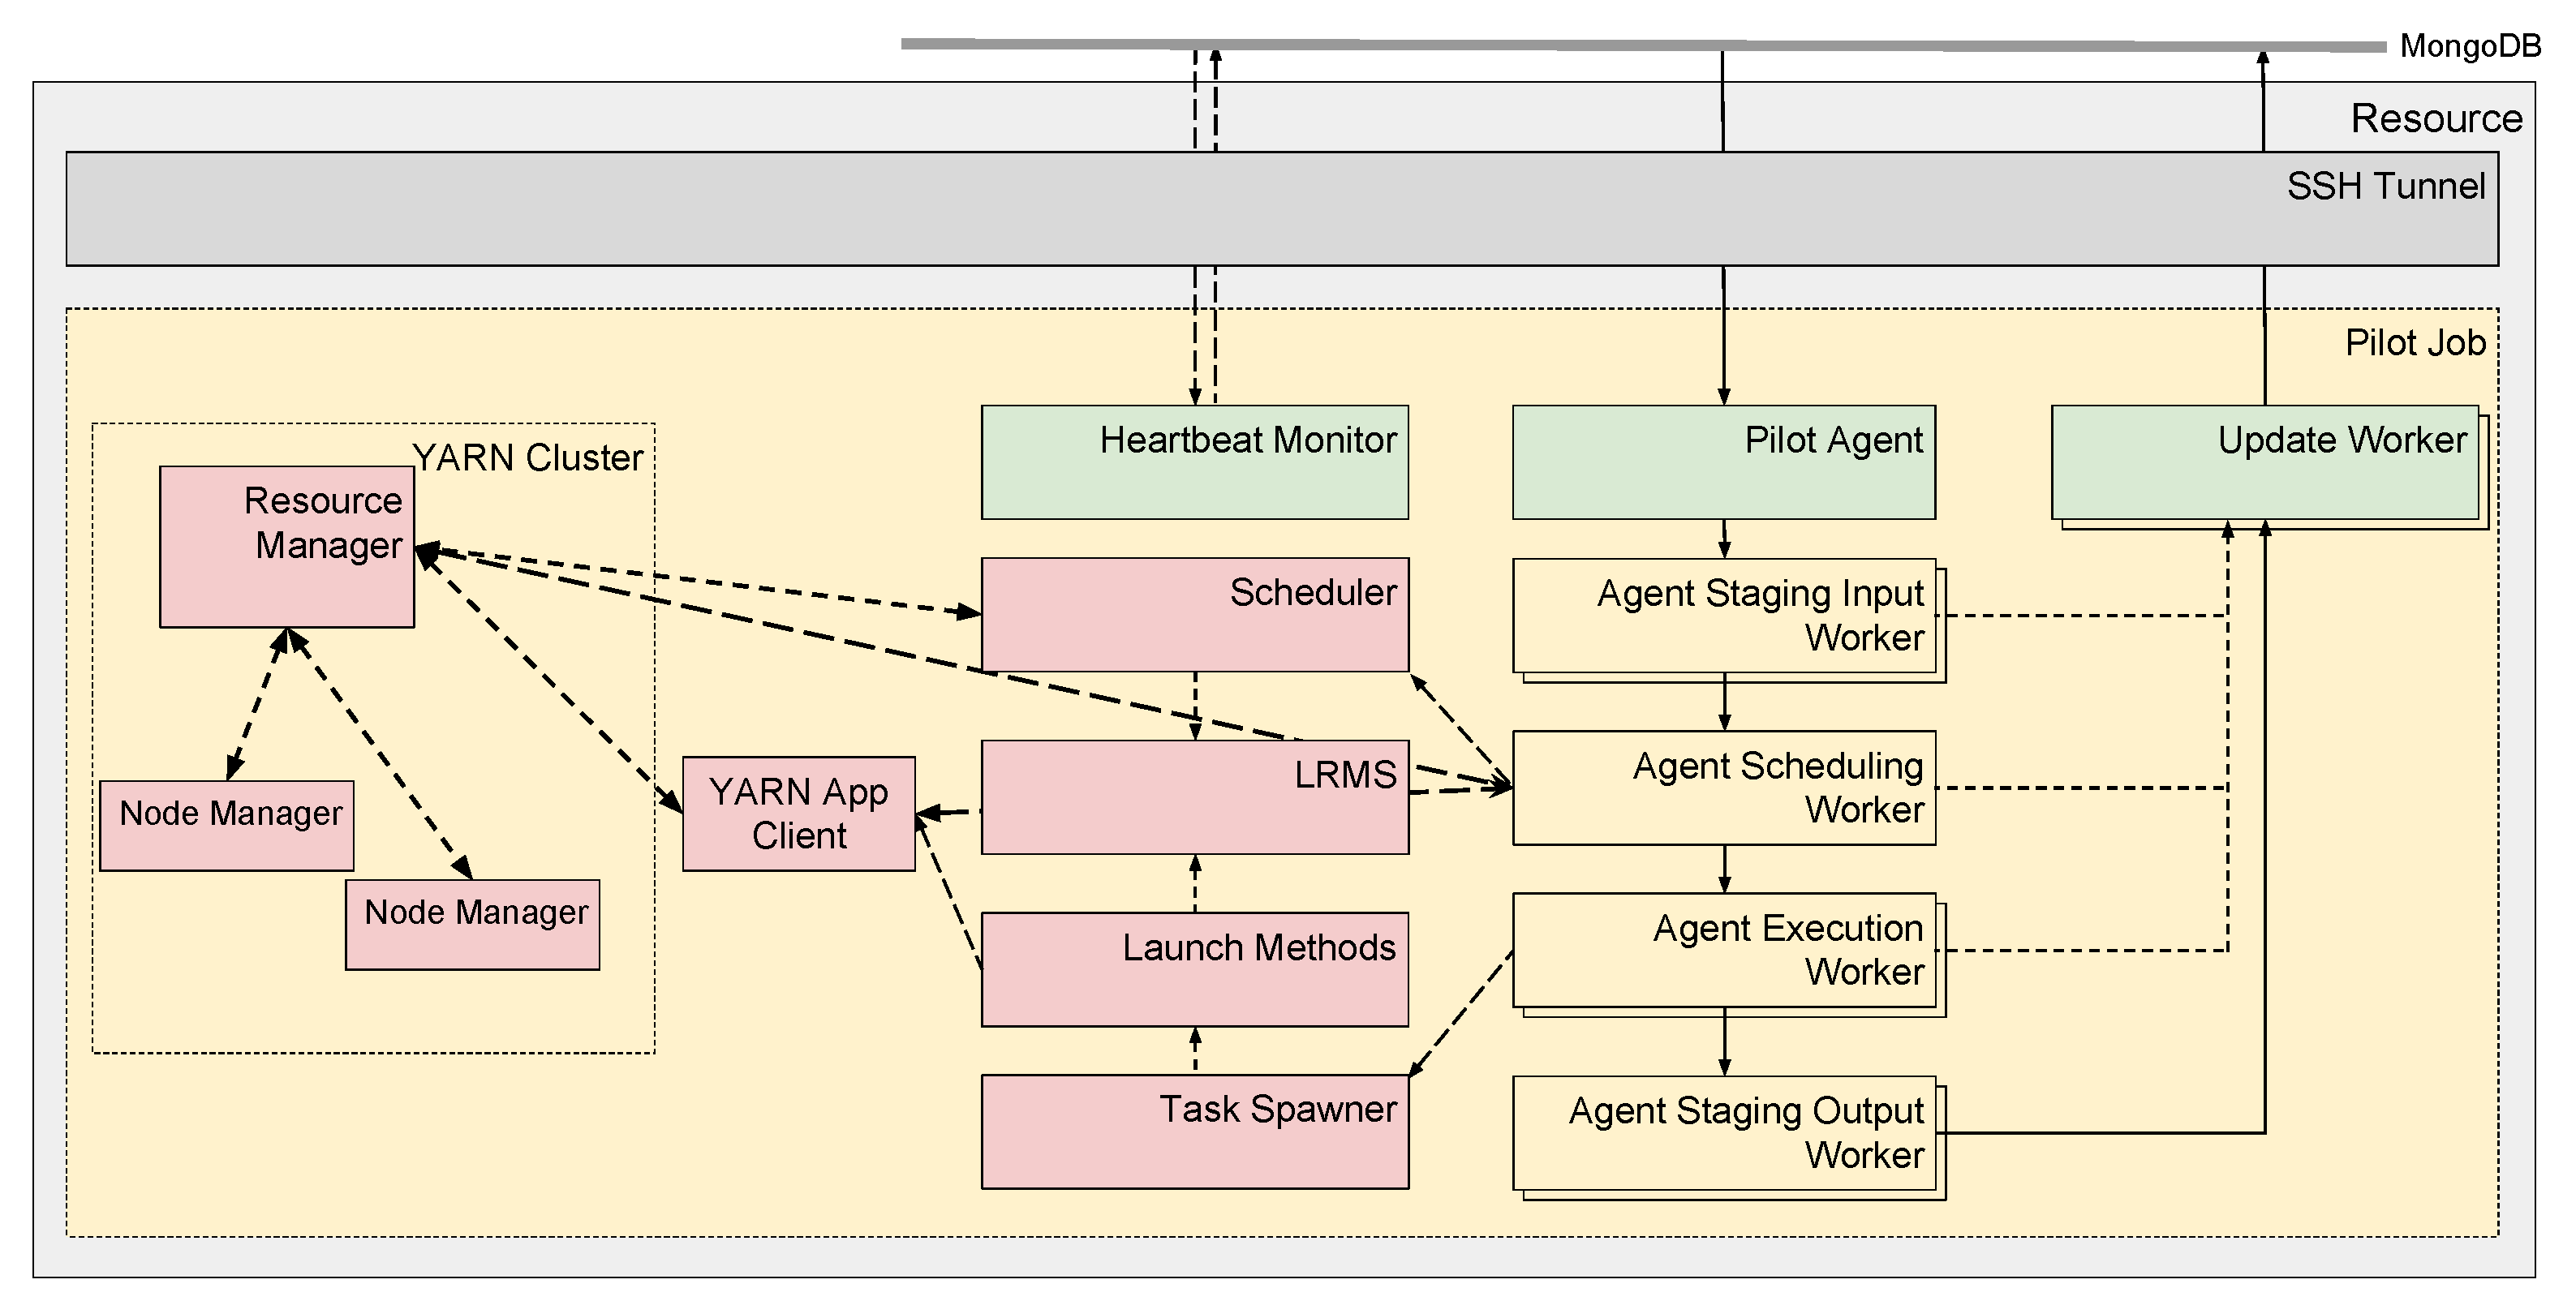
\includegraphics[scale=.22]{RP_YARN_Interaction_Diagram.pdf}
			\caption{The interaction between RADICAL-Pilot and YARN. As seen in \cite{hadoop_paper}.}
			\label{fig:rp_yarn_interaction}
		\end{figure}

		These changes, among others, give RADICAL-Pilot-YARN the dual functionalities tat are so desirable for those users working with compute- and data-intensive simulations. 

\section{Experiments}

	\subsection{EnsembleMD Analysis}
		The performance experiments described in this section were designed to analyze the Pipeline and Simulation Analysis Patterns. We define the experiment configurations, and explain useful diagrams here.

		\subsubsection{Algorithm and Configuration}
			The experiment is comprised of a two-stage workload; the first stage consists of creating a 10Mb file of random characters, and the second stage performs a character count on this file. In Table \ref{table:kernel_execution_table}, we have included the commands used to execute each stage as well as the average execution time from the Bash Shell. We also use the environment parameters specified in Table \ref{table:environment_variables}.

			\begin{table}[H]
				\centering
				\begin{tabu}{|c|c|c|}
					\hline
					Kernel & Bash Command & Avg. Execution (seconds) \\
					\hline
					misc.mkfile & base64 /dev/urandom | & .008 \\ 
								& head -c 100 > test.txt  \\
					\hline
					misc.ccount & grep -o . test.txt |  & .004\\ 
								& sort | uniq > out.txt   \\
					\hline
				\end{tabu}
				\caption{Kernels, their commands, and their expected execution times.}
				\label{table:kernel_execution_table}
			\end{table}

			\begin{table}[H]
				\centering
				\begin{tabular}{|c|c|}
						\hline
						Parameter & Value \\
						\hline
						\hline
						EnsembleMD-Toolkit version & 0.3.14-27-g65bc062 \\
						\hline
						EnsembleMD Branch & devel \\
						\hline
						RADICAL-Pilot version & 0.40.1 \\
						\hline
						Target Machine & XSEDE Stampede \\
						\hline
				\end{tabular}
				\caption{Environment Parameters.}
				\label{table:environment_variables}
			\end{table}

			To examine the performance of the Toolkit, we measure the duration of several key components of the execution. These components are defined in Table \ref{table:measured_components}.

			\begin{table}[H]
				\centering
				\begin{tabular}{|c|p{10cm}|}
						\hline
						Component & \multicolumn{1}{|c|}{Definition} \\
						\hline
						\hline
						EnsembleMD Core Overhead & Overhead incurred by EnsembleMD Toolkit when allocating and deallocating a cluster. \\
						\hline
						Data Movement &  Overhead incurred in moving input data from the local machine to remote node, and from moving the output data from the remote node to the local machine\\
						\hline
						X Execution Time & Total time required to complete phase X of the Pattern\\
						\hline
						RADICAL-Pilot Overhead & Overhead incurred by the underlying RADICAL-Pilot API \\
						\hline
				\end{tabular}
				\caption{Measured Components}
				\label{table:measured_components}
			\end{table}

			We then place timestamps at appropriate places in the pilot's execution corresponding to each of these components, as shown in Figure \ref{fig:param_pilot_state_mapping}.

			% Param/State Mapping
			\begin{figure}[H]
				\centering
				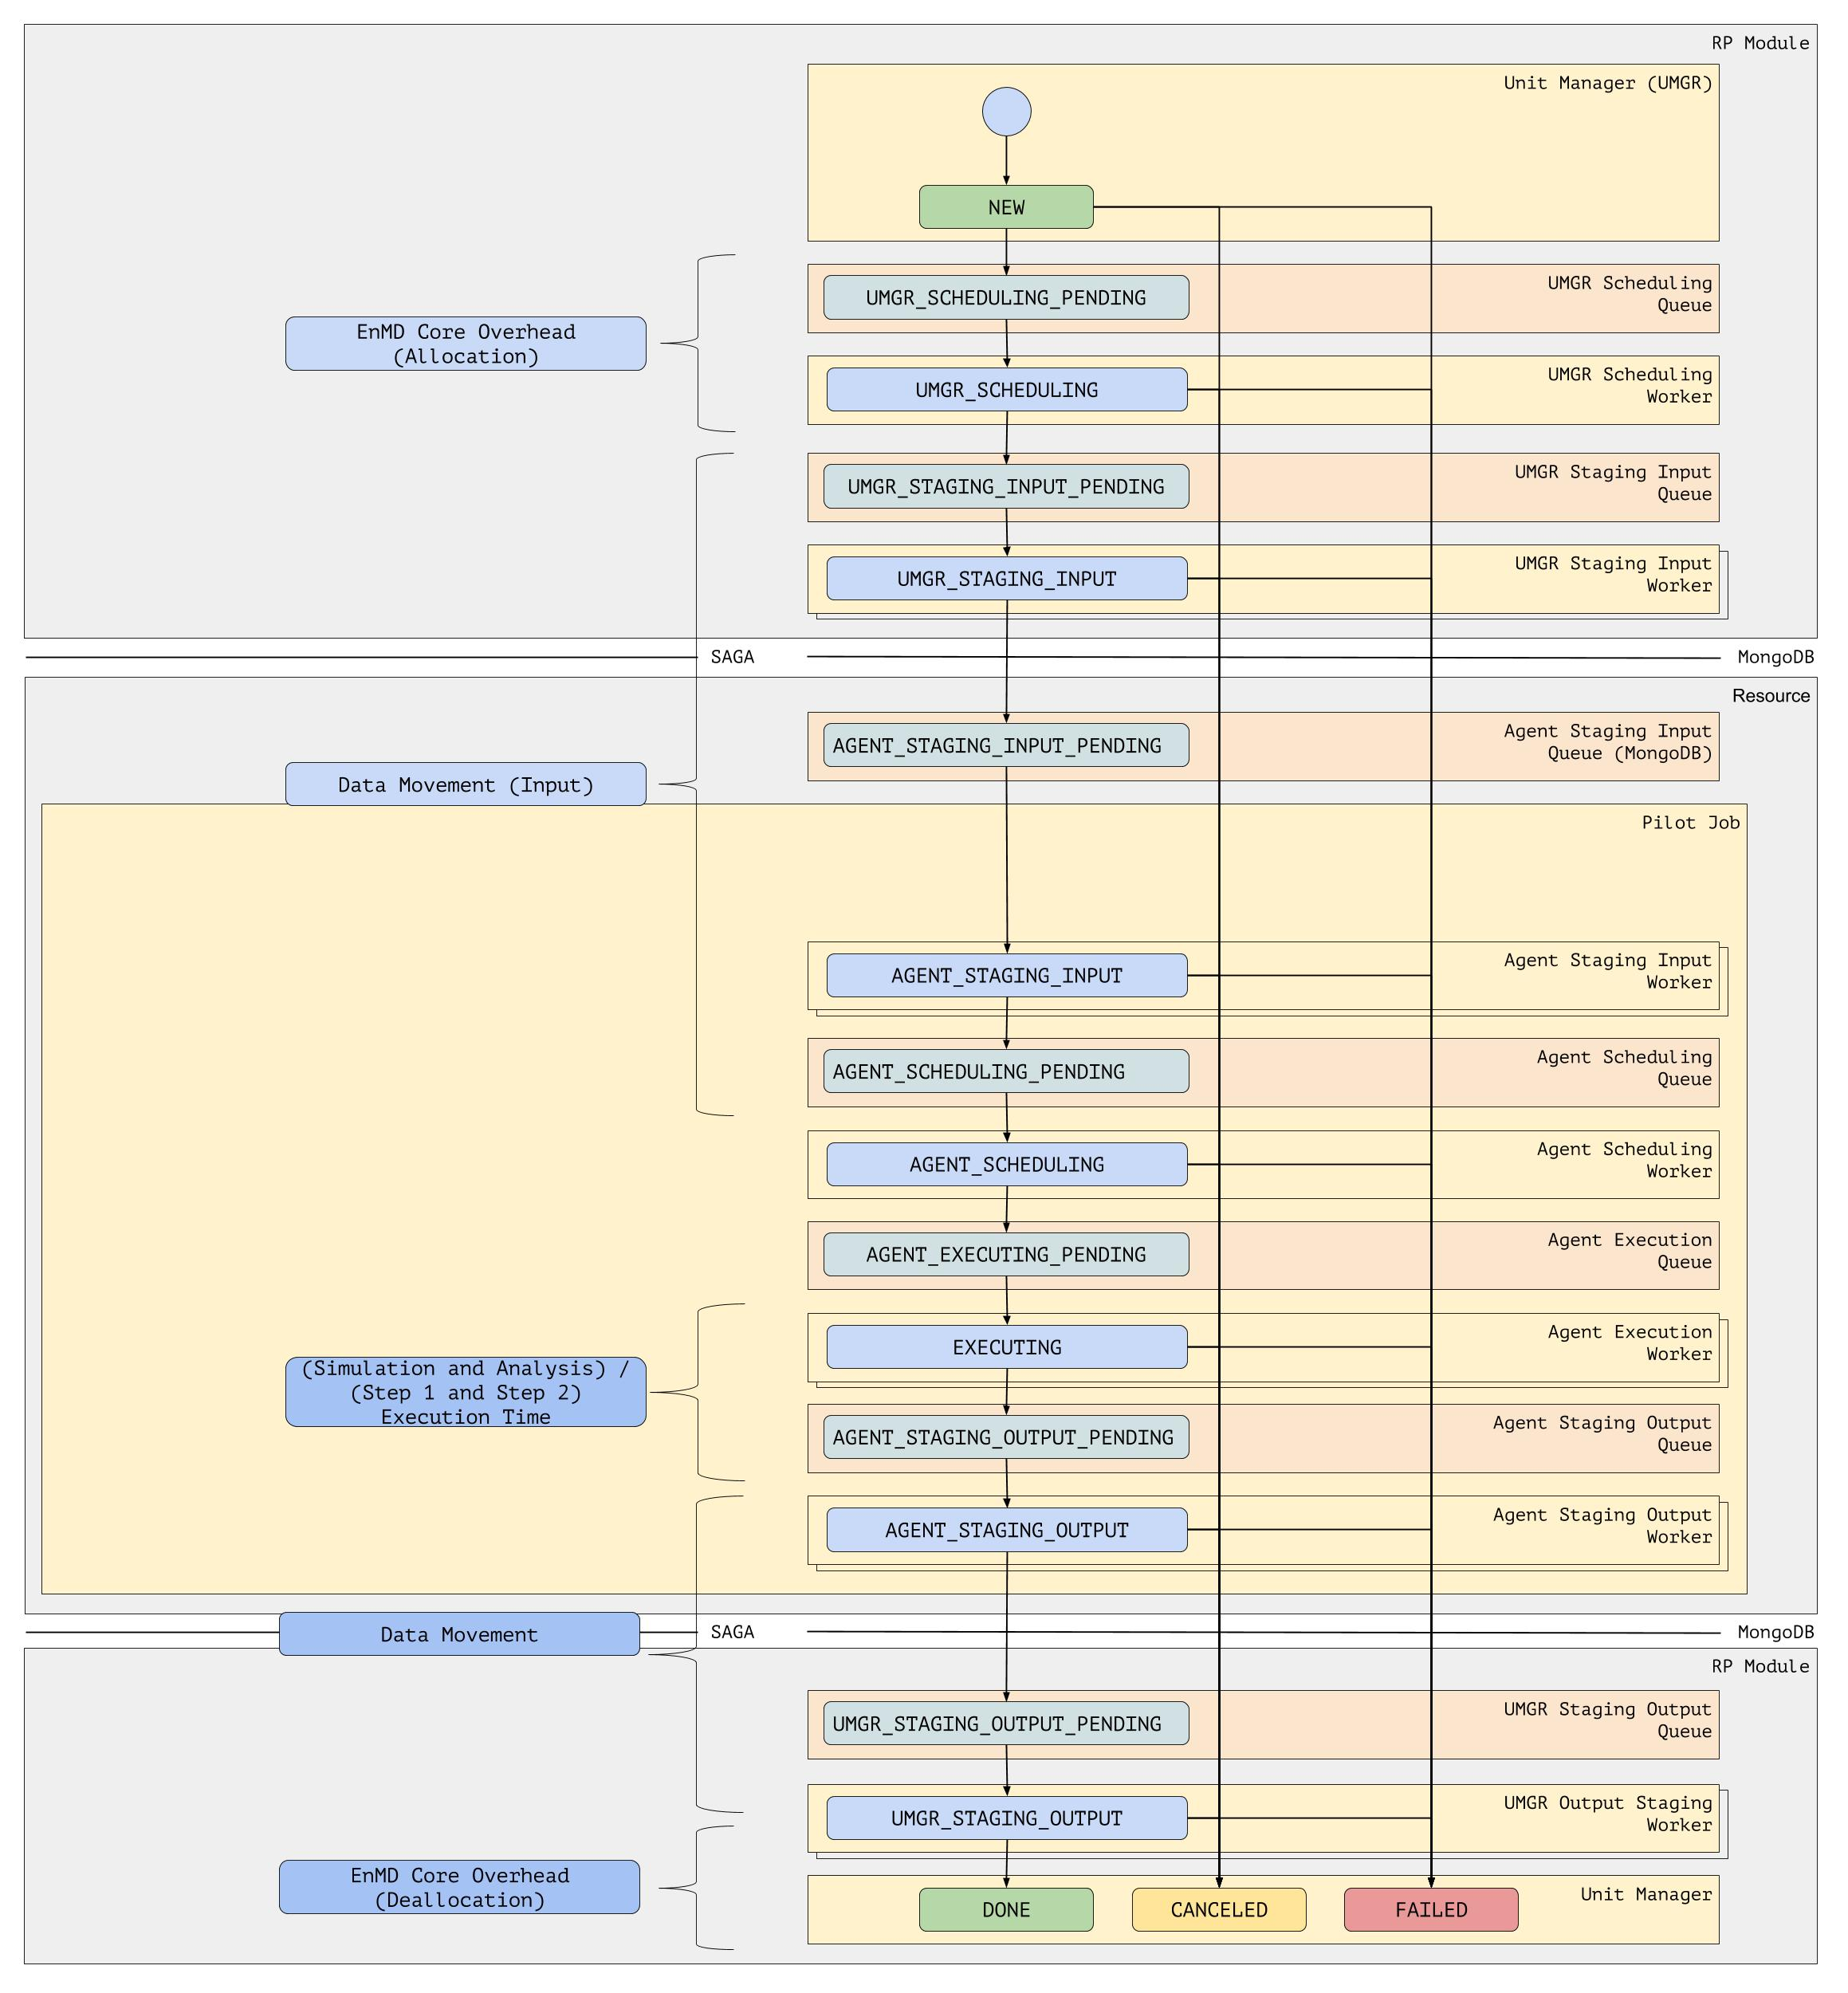
\includegraphics[scale=.10]{enmd_state_model_mapping.jpg}
				\caption{Mapping of parameters to pilot state model. Derived from \cite{rp_state_diagram}.}
				\label{fig:param_pilot_state_mapping}
			\end{figure}


			Each of the components exhibited in Figure \ref{fig:param_pilot_state_mapping} is governed differences in timestamps. The following equations explicitly describe those differences.

			\begin{align*}
				EnMD Core Overhead = (alloc\_stop - alloc\_start) + (dealloc\_stop - dealloc\_start) \numberthis \label{1}
			\end{align*}

			\begin{align*}
				EnMD Pattern Overhead = &(step1\_wait-step1\_start) + (step1\_stop - step1\_res) + \numberthis \label{2} \\
										&(ana\_wait-ana\_start) + (ana\_stop - ana\_res) 
			\end{align*}

			\begin{align*}
				RP Overhead = &((step1\_wait - step1\_res) - step1\_data\_movement - step1\_execution\_time) + \\ \numberthis \label{3} 
							  &((ana\_wait - ana\_res) - ana\_data\_movement - ana\_execution\_time) 
			\end{align*}

			\begin{align*}
				Data Movement = &((step1\_Done - step1\_PendingAgentOutputStaging) + \\
								&(step1\_Allocating - step1\_StagingInput)) + \numberthis \label{4} \\
								&((ana\_Done - ana\_PendingAgentOutputStaging) + \\
								&(ana\_Allocating - ana\_StagingInput)) 
			\end{align*}
			
			\begin{align*}
				Step 1 Execution Time = PendingAgentOutputStaging - Executing \numberthis \label{5}
			\end{align*}

			\begin{align*}
				Step 2 Execution Time = PendingAgentOutputStaging - Executing \numberthis \label{6}
			\end{align*}

			\begin{align*}
				EnMD Pattern Overhead = &(sim\_wait-sim\_start) + (sim\_stop - sim\_res) + \numberthis \label{7} \\
										&(ana\_wait-ana\_start) + (ana\_stop - ana\_res) 
			\end{align*}

			\begin{align*}
				RP Overhead = &((sim\_wait - sim\_res) - sim\_data\_movement - sim\_execution\_time) + \\ \numberthis \label{8} 
							  &((ana\_wait - ana\_res) - ana\_data\_movement - ana\_execution\_time) 
			\end{align*}

			\begin{align*}
				Data Movement = &((sim\_Done - sim\_PendingAgentOutputStaging) + \\
								&(sim\_Allocating - sim\_StagingInput)) + \numberthis \label{9} \\
								&((ana\_Done - ana\_PendingAgentOutputStaging) + \\
								&(ana\_Allocating - ana\_StagingInput)) 
			\end{align*}
			
			\begin{align*}
				Simulation Execution Time = PendingAgentOutputStaging - Executing \numberthis \label{10}
			\end{align*}

			\begin{align*}
				Analysis Execution Time = PendingAgentOutputStaging - Executing \numberthis \label{11}
			\end{align*}



			Figures ~\ref{fig:pattern_rp_overheads} details the measurements taken within the Execution Time state shown in Figure ~\ref{fig:param_pilot_state_mapping}. The start and stop times indicate when execution starts and ends for that particular stage. The wait time indicates when the stage submits all of its tasks and waits for them to finish. Finally, the ``res time'' is defined as the point when all tasks of that stage have finished execution and the EnMD Toolkit resumes execution to prepare for the next stage. The terms in the parenthesis, (step1/sim) and (ana/ana), do not indicate division; this notation is used to condense the Pipeline Overhead diagram and the Simulation Analysis Overhead diagram into one figure. In the Pipeline case, the diagrams would include the ``step1'' and ``ana'' terms, whereas the Simulation Analysis case would include the ``sim'' and ``ana'' terms. Similarly, we defined separate but very similar equations to measure the components; equations 2 thorugh 6 are specific to the Pipeline pattern, whereas equations 7 through 11 are specific to the Simulation-Analysis pattern.

			\begin{figure}[H]
				\centering
				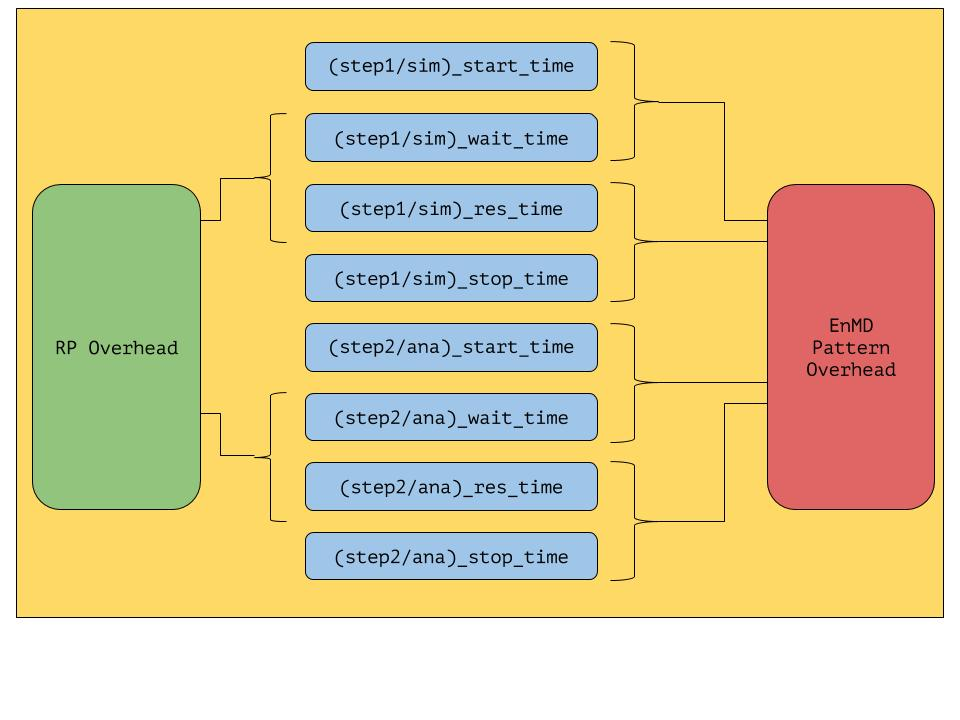
\includegraphics[scale=.28]{pattern_and_rp_overheads.jpg}
				\caption{EnMD and RP Overheads. Derived from \cite{rp_state_diagram}.}
				\label{fig:pattern_rp_overheads}
			\end{figure}

		\subsubsection{Types of Scaling}
			For these experiments, we measured performance as a function of the number of cores allocated to a script as well as the number of instances of the Pattern being executed. We initially implemented weak scaling, in which the number of cores scales at the same rate as the number of instances, with the goal of observing a relatively constant execution time. The intuition behind this is that the core to instance ratio stays the same, which implies that the work per core/instance combination is the same. We also perform strong scaling, in which we hold the number of instances constant while we scale the number of cores. In this case, we expect that the Pattern will make use of the additional cores to finish the task more quickly. The scale that we use for these experiments is [1,16,32,64,128].

			In each script, we measured the time taken to complete various stages of execution. These will be elaborated upon in the subsection for each pattern.

		\subsubsection{Pipeline}
			For the Pipeline pattern, we measured the parameters defined in equations 2 through 6. 

			% Pipeline Weak Scaling
			\begin{figure}[H]
				\centering
				% 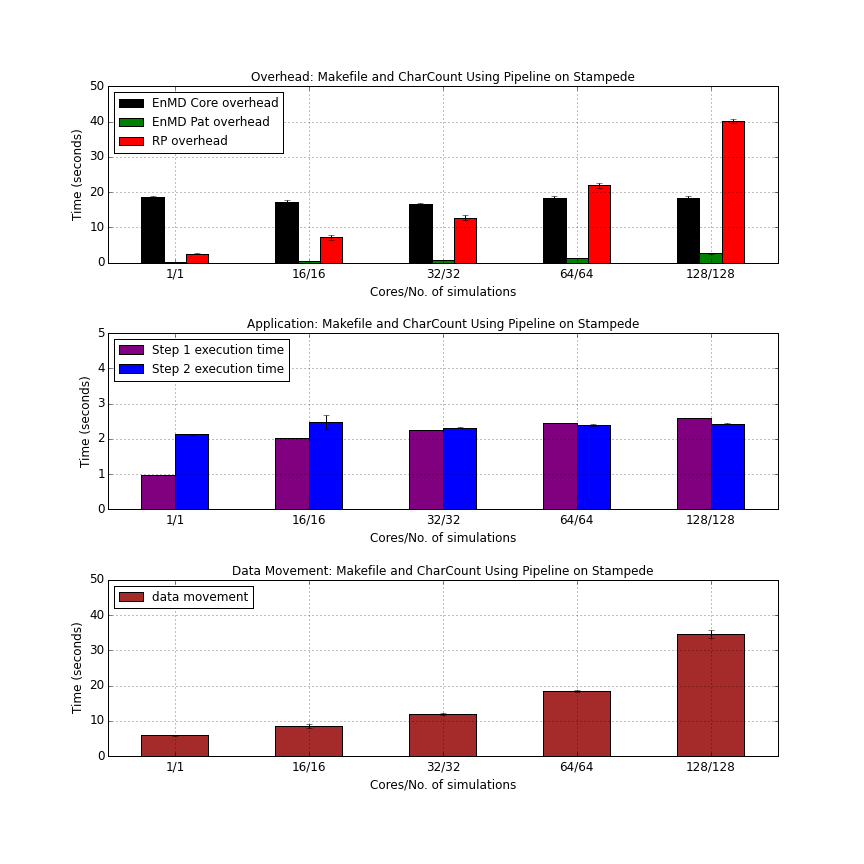
\includegraphics[scale=.30]{pipeline_weak_scaling.png}
				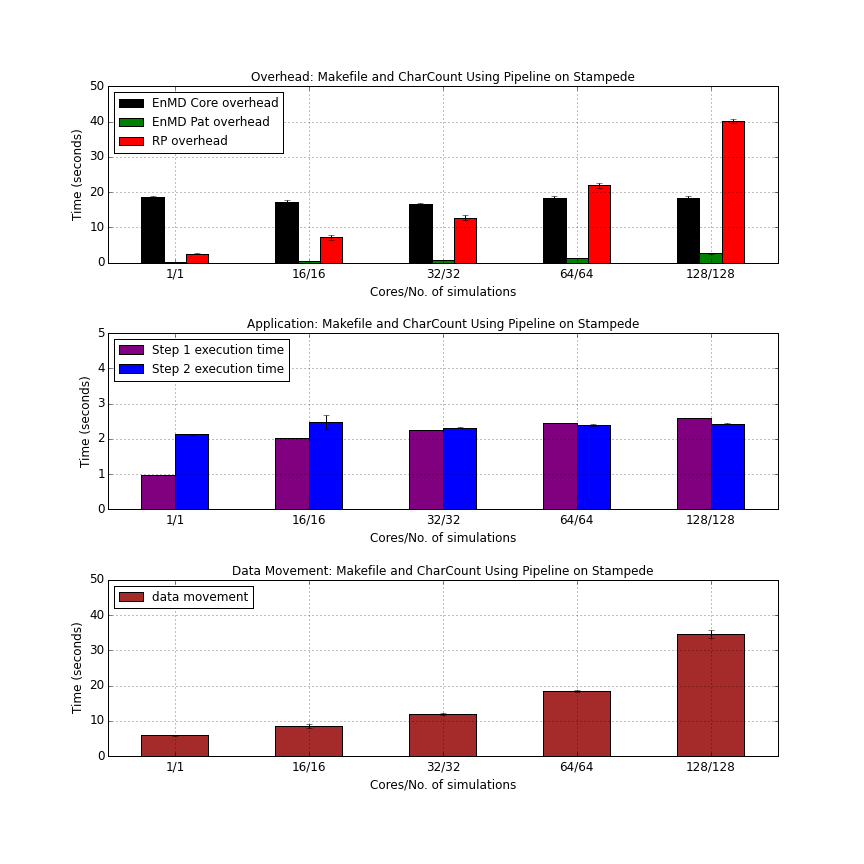
\includegraphics[width = 9cm, height = 8cm]{pipeline_weak_scaling.png}
				\caption{Weak Scaling with the Pipeline Pattern}
				\label{fig:pipeline_weak_scaling}
			\end{figure}

			Figure ~\ref{fig:pipeline_weak_scaling} shows the scaling behavior of each of the parameters. In the first graph, we observe that the EnsembleMD Core overhead stays relatively constant at about 18 seconds throughout the scaling. We also see that the EnsembleMD Pattern Overhead is at most 3 seconds, which is a fraction of the Core overhead. Finally, we see that the RADICAL-Pilot overhead increases rapidly as the scale increases. Ratios between RP overheads from a configuration to the previous configuration yield a value of about 1.8, which implies that the overhead is growing linearly.
			In the second graph of Figure 1, we see that the execution times for both Step 1 and Step 2, which were the Makefile and Character Count respectively, stay very much constant throughout the scaling, except for the anomaly of Step 1 in the first configuration. This is to be expected, as the settings in the configuration should have no effect on how long it takes to run the underlying Bash commands. However, the times shown are much larger than those observed when the commands are executed directly from a Bash prompt. It is possible that the extra time is due to overhead from a combination of EnsembleMD and RADICAL-Pilot, but we have not dissected this additional component.
			Finally, the data movement shows a steady increase in duration. The ratios from one configuration to the previous configuration fluctuate from 1.6 to 1.9, but generally imply a linear increase as a function of the number of cores and execution instances. 


			\begin{figure}[H]
				\centering
				% \includegraphics[scale=.25]{img/pipeline_strong_scaling.png}
				\includegraphics[width = 10cm, height = 9cm]{pipeline_strong_scaling.png}
				\caption{Strong Scaling with the Pipeline Pattern}
				\label{fig:pipeline_strong_scaling}
			\end{figure}

			Figure ~\ref{fig:pipeline_strong_scaling} displays the strong scaling results from the Pipeline. Looking at the EnsembleMD Core Overhead, we find that it averages to around 22 seconds. On the other hand, the Pattern Overhead was measured at 15ms on average, so the values at each configuration did not register on the scale of the Core Overhead. The RP overhead remains approximately constant at around 8 seconds. The execution times for Steps 1 and 2 show a much different trend than they did in the weak scaling experiments; in general, Step 1 showed execution times that were closer to the actual execution time, but were still three orders of magnitude greater. Step 2 fluctuated much more than it did during the weak scaling experiments.
			Data movement shows a general decline in duration, aside from the anomaly with 64 cores. This may be due to the increased number of cores available for the movement.

		\pagebreak
		\subsubsection{Simulation Analysis}

			For Simulation Analysis, we considered the parameter definitions in equations 7 through 11.

			\begin{figure}[H]
				\centering
				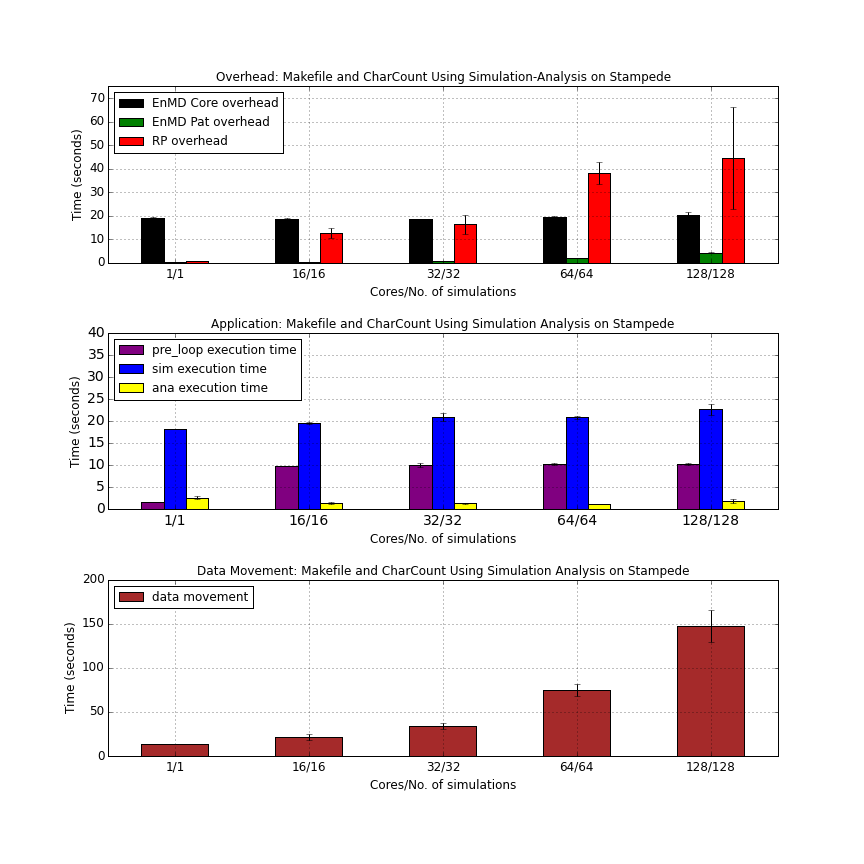
\includegraphics[scale=.29]{sa_weak_scaling.png}
				\caption{Weak Scaling with the Simulation Analysis Pattern}
				\label{fig:sa_weak_scaling}
			\end{figure}

			In Figure ~\ref{fig:sa_weak_scaling}, we see scaling behavior similar to what we saw in the original pipeline weak scaling experiment. The EnsembleMD Core Overhead is essentially constant, the Pattern Overhead is small in comparison and is capped at around 5 seconds, and the RP overhead does show an increase across the combinations. However, the RADICAL-Pilot overhead does not show a distinct linear progression in the same fashion as the Pipeline Weak Scaling plot did. 
			The second plot shows the phases of execution of the experiment. The pre-loop phase contained no logic, so our inference is that the times shown are the overhead introduced to make the call to the pre-loop. The Simulation execution time, which contained the Makefile Kernel, was constant throughout the scaling, but took longer on average than it did for the Pipeline. The Character Count, encapsulated by the Analysis stage, was truer to the values recorded in the Pipeline Weak Scaling plot.
			The Data movement plot shows a similar increase in the time needed to download the output data, but the trend does not seem to be linear. 

			\begin{figure}[H]
				\centering
				% 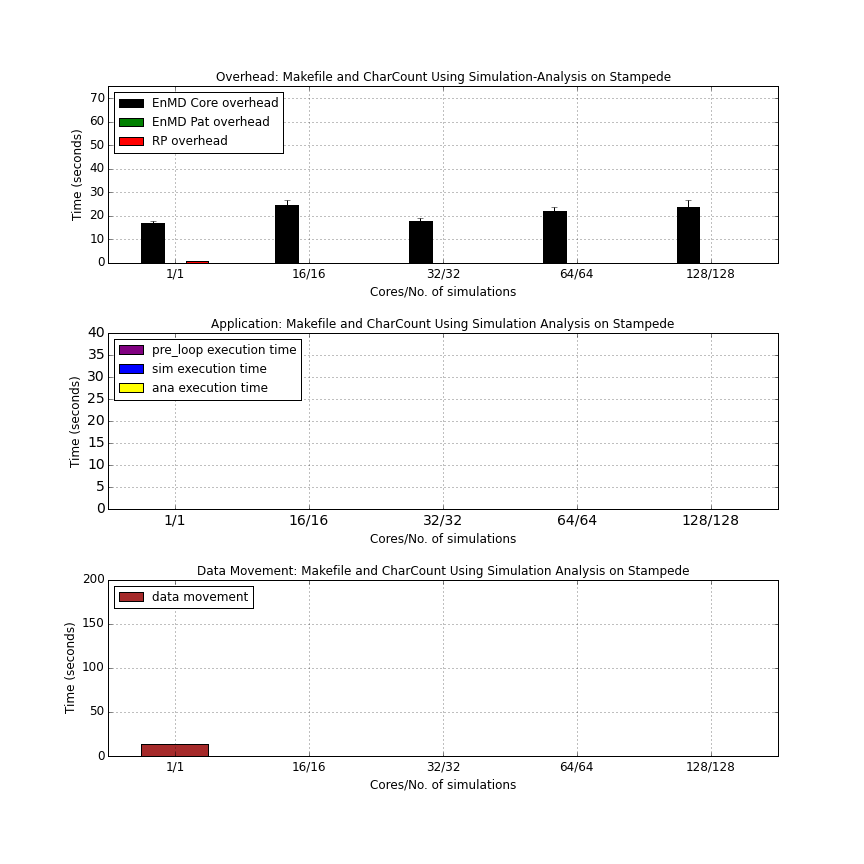
\includegraphics[scale=.30]{sa_strong_scaling.png}
				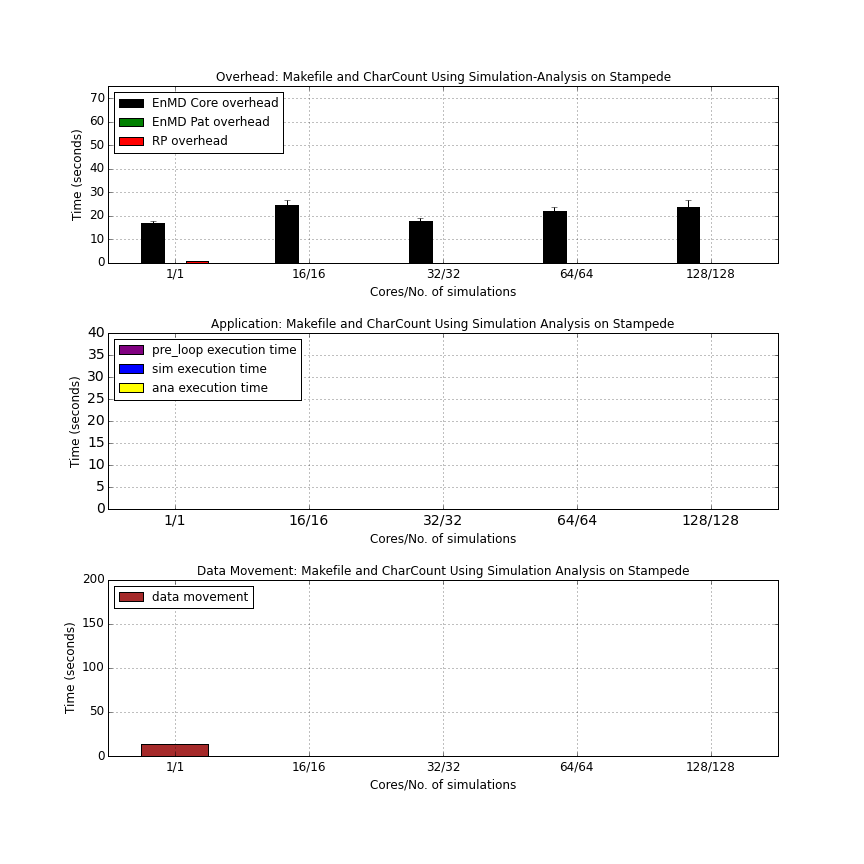
\includegraphics[width = 8cm, height = 9cm]{sa_strong_scaling.png}
				\caption{Strong Scaling with the Simulation Analysis Pattern}
				\label{fig:sa_strong_scaling}
			\end{figure}
			
			Finally, we examine the behaviors of each measurement during the Strong Scaling experiments with Simulation Analysis in Figure ~\ref{fig:sa_strong_scaling}. EnsembleMD Core Overhead wavers around 20 seconds, whereas the RADICAL-Pilot Overhead has a large amount of variation in its time. Again, the EnsembleMD Pattern Overhead averages to approximately 20ms, and thus are not be visible on the same graph.
			In the Simulation phase, we find that the execution time has been reduced dramatically, and that a representative value for it could be 13ms. The Analysis phase also varies slightly, but can be approximated at 7ms.
			The Data Movement durations are troubling, seeing as there is not a clear pattern to how the different values were obtained. The scaling does not seem to have had a visible effect on the duration of this phase.

	\subsection{RADICAL-Pilot/RADICAL-Pilot-YARN Analysis}
		Our experiments to compare the two softwares involve running the K-means algorithm using a varying number of clusters and points in order to judge performance capabilities. We first summarize the algorithm, and then detail the experiment configuration in Table \ref{table:config_table}.

		\subsubsection{Algorithm and Configuration}
			The K-means algorithm seeks to iteratively classify a set of data points in to k different clusters. It starts by placing k centroids as far away from each other as possible, but still making a first approximation of the possible classifications. Then every data point is assigned to the nearest centroid based on distance. Once this is done, a new set of k centroids is determined based on the previous assignments \cite{k_means}. Over many iterations, the centroids will eventually converge to their proper locations. The iteration is done by minimizing an error function:

			\[ J = \sum_{j=1}^{k} \sum_{i=1}^{n} \lVert \textbf{x}_{i}^{(j)} - \textbf{c}_j \rVert ^ 2\]

			where $\lVert \textbf{x}_{i}^{(j)} - \textbf{c}_j \rVert ^ 2$ represents the distance between centroid $\textbf{c}_j$ and the data point $\textbf{x}_{i}^{(j)}$. The result are k different points that represent the optimal classifications fo the data set.

			\begin{table}[H]
				\centering
				\begin{tabu}{|c|c|}
					\hline
					Parameter & Value \\ 
					\hline
					\hline
					RADICAL-Pilot Version & v0.40.1-41-g6101f4a \\
					\hline
					Target Machine & XSEDE Stampede \\ 
					\hline
					Iterations of K-Means & 2\\ 
					\hline
					Cores & [8,16,32]\\
					\hline
					Tasks & [8,16,32]\\
					\hline
					Clusters & [50,500,5000] \\
					\hline
					Total Data Points & [10000,100000,1000000]\\
					\hline
					Data sets & \url{dataset_100K_3d.in}, \url{dataset_10K_3d.in}, \url{dataset_1M_3d.in}\\
					\hline
				\end{tabu}
				\caption{Experiment Parameters}
				\label{table:config_table}
			\end{table}

			% Explanation of Parameters
			Table \ref{table:config_table} shows the parameters involved in this experiment. We implement the k-Means algorithm on XSEDE's Stampede machine using RADICAL-Pilot version 0.40.1, and we run two iterations of the algorithm. We want the computational cost of the experiment to remain the same in each configuration, so we constrain the product of the number of clusters and the number of data points to be constant. Doing this, we run the algorithm on configurations of 50 clusters and 1,000,000 points, 500 clusters and 100,000 points, and 5000 clusters and 10,000 points. Each of these points is represented by a vector of length three, which is commonly used to describe the locations and velocities of particles in three dimensional space. We run each configuration using 8, 16, and 32 cores each, and we set the number of tasks equal to the number of cores. Finally, we run this entire configuration using both RADICAL-Pilot and RADICAL-Pilot-YARN. This set up of the experiment allows us to examine the scaling behavior of both softwares in terms of the number of cores, and to compare the performance of each under identical conditions.

			% Pilot-State Mapping
			In this experiment, we only track the time-to-completion for each software. Measuring individual components is not necessary here, as the experiment is intended to present the two softwares as black boxes and requires the user to pay attention only to how fast his script is completed. However, one can see what states the time-to-completion measurement encompasses in Figure \ref{fig:pilot_state_mapping}.

			\begin{figure}[H]
				\centering
				% 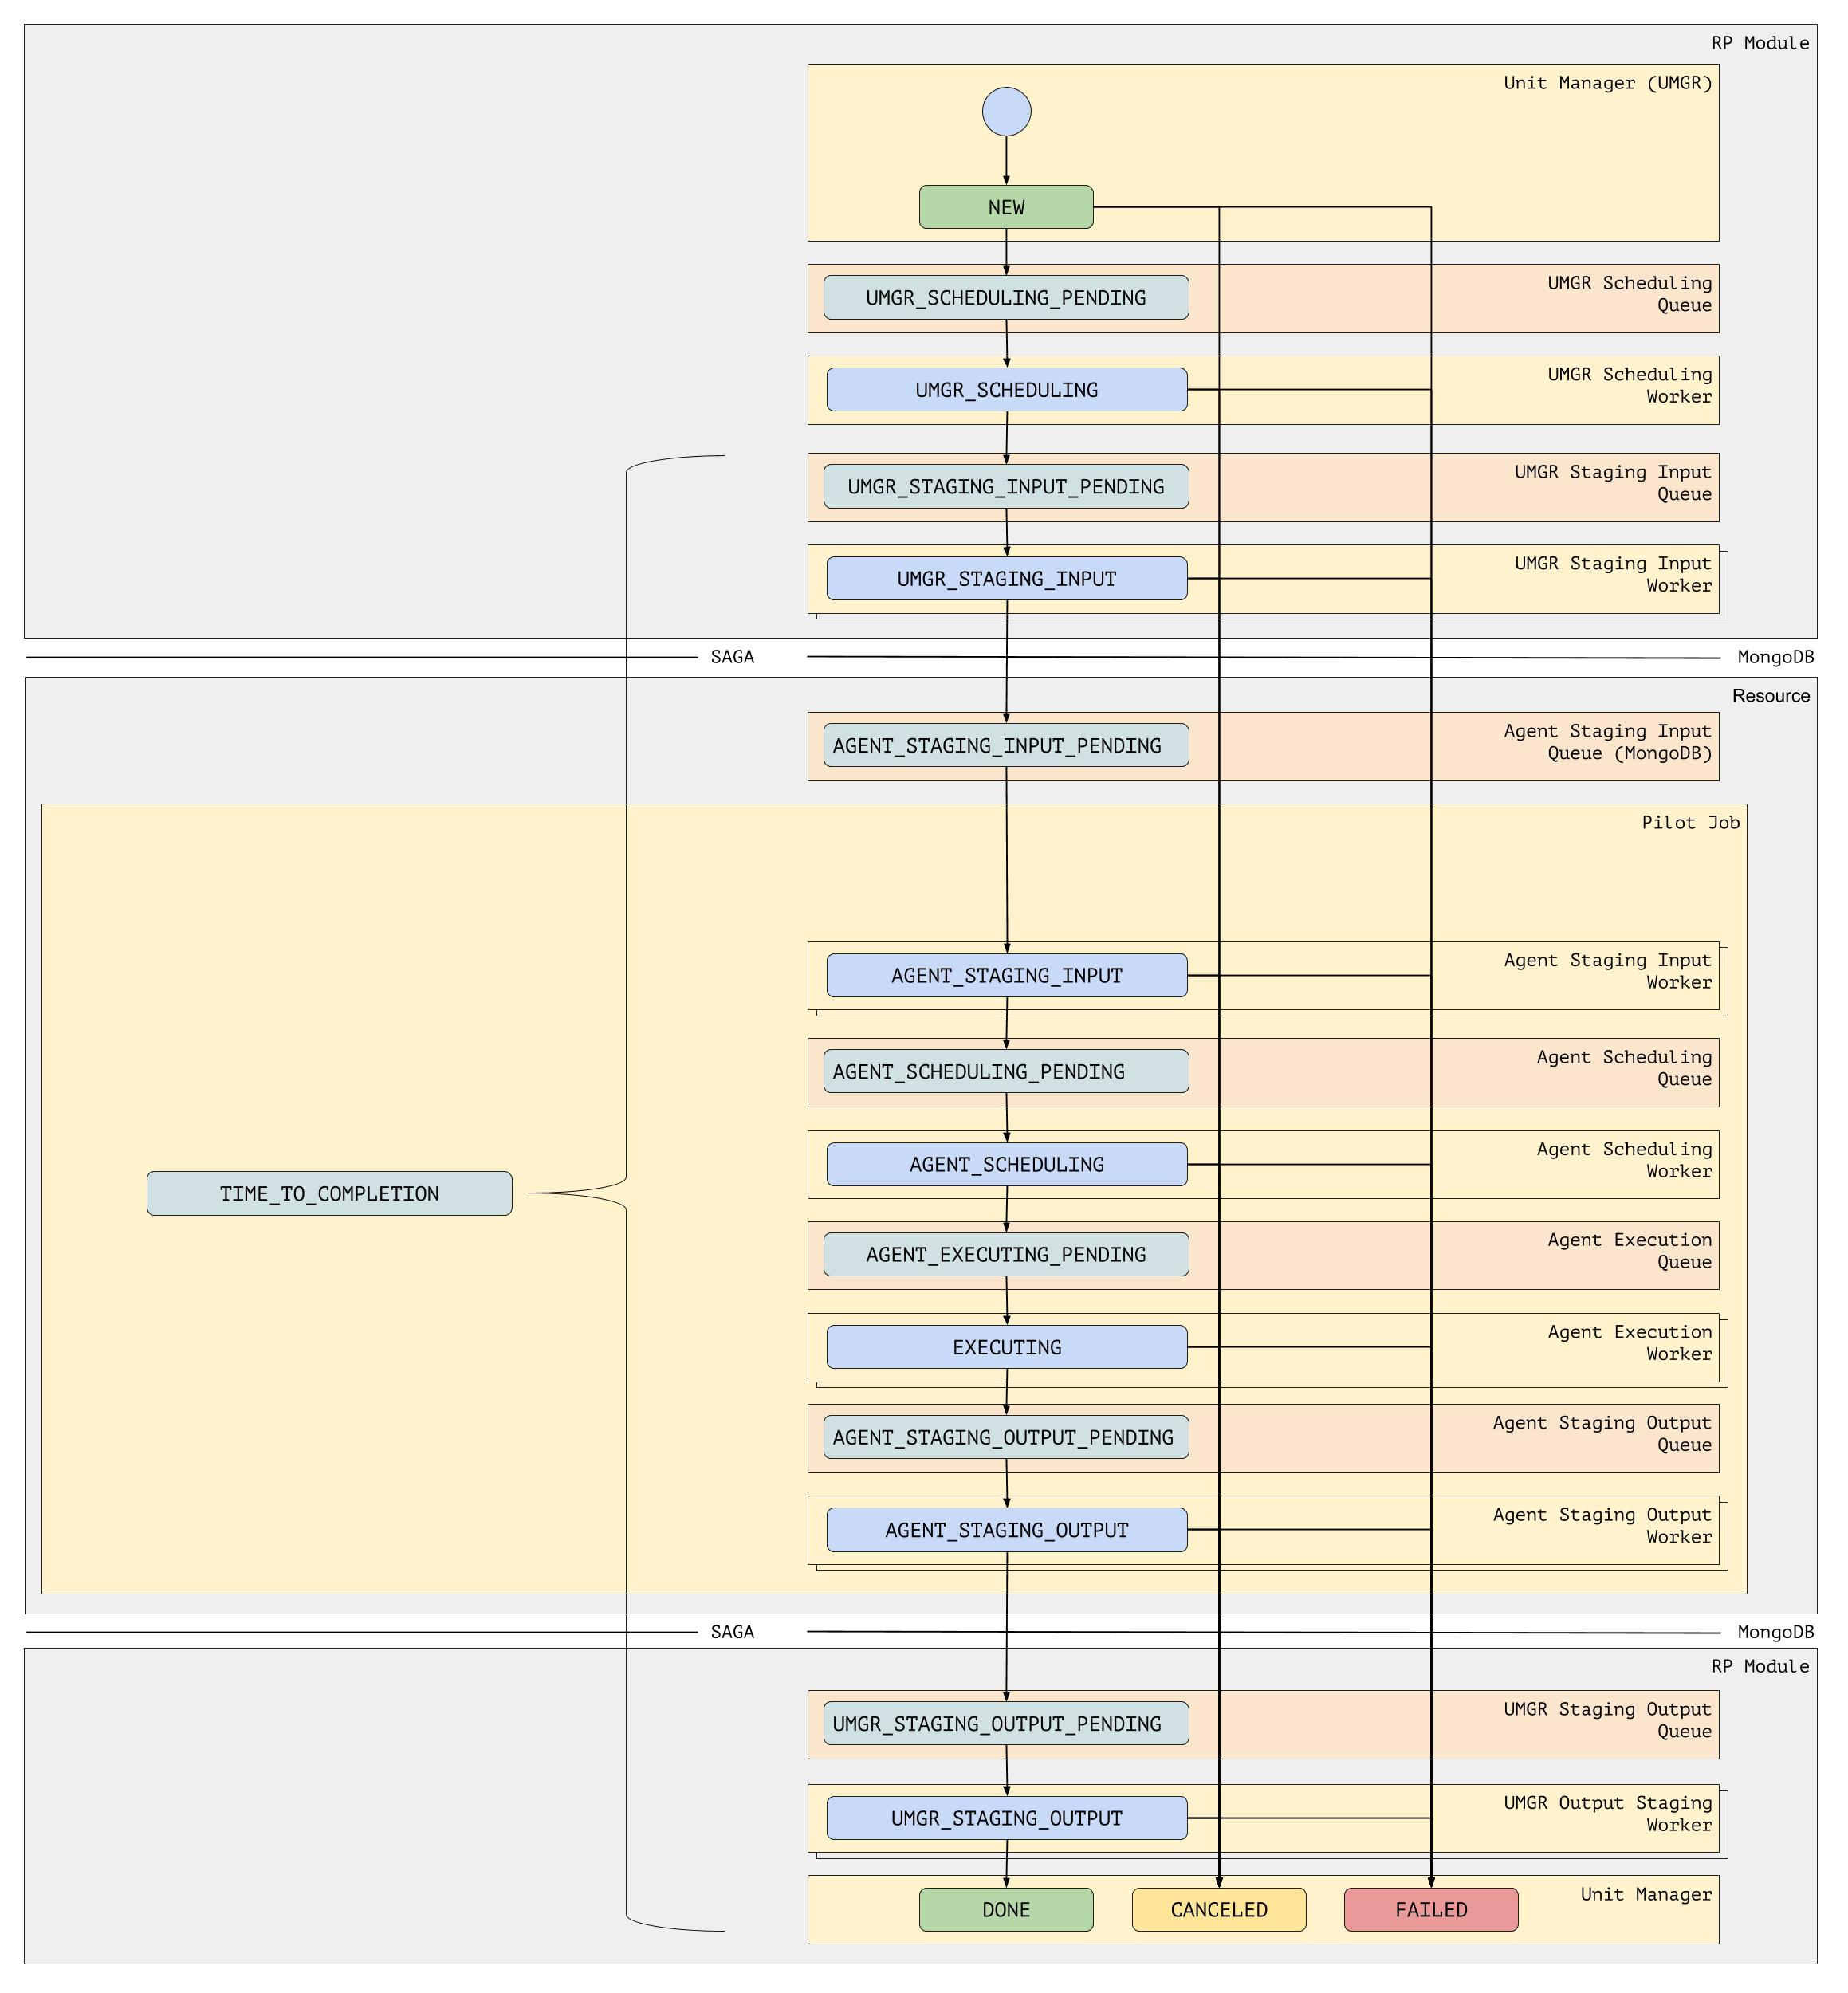
\includegraphics[scale=.19]{rp_state_model_mapping.jpg}
				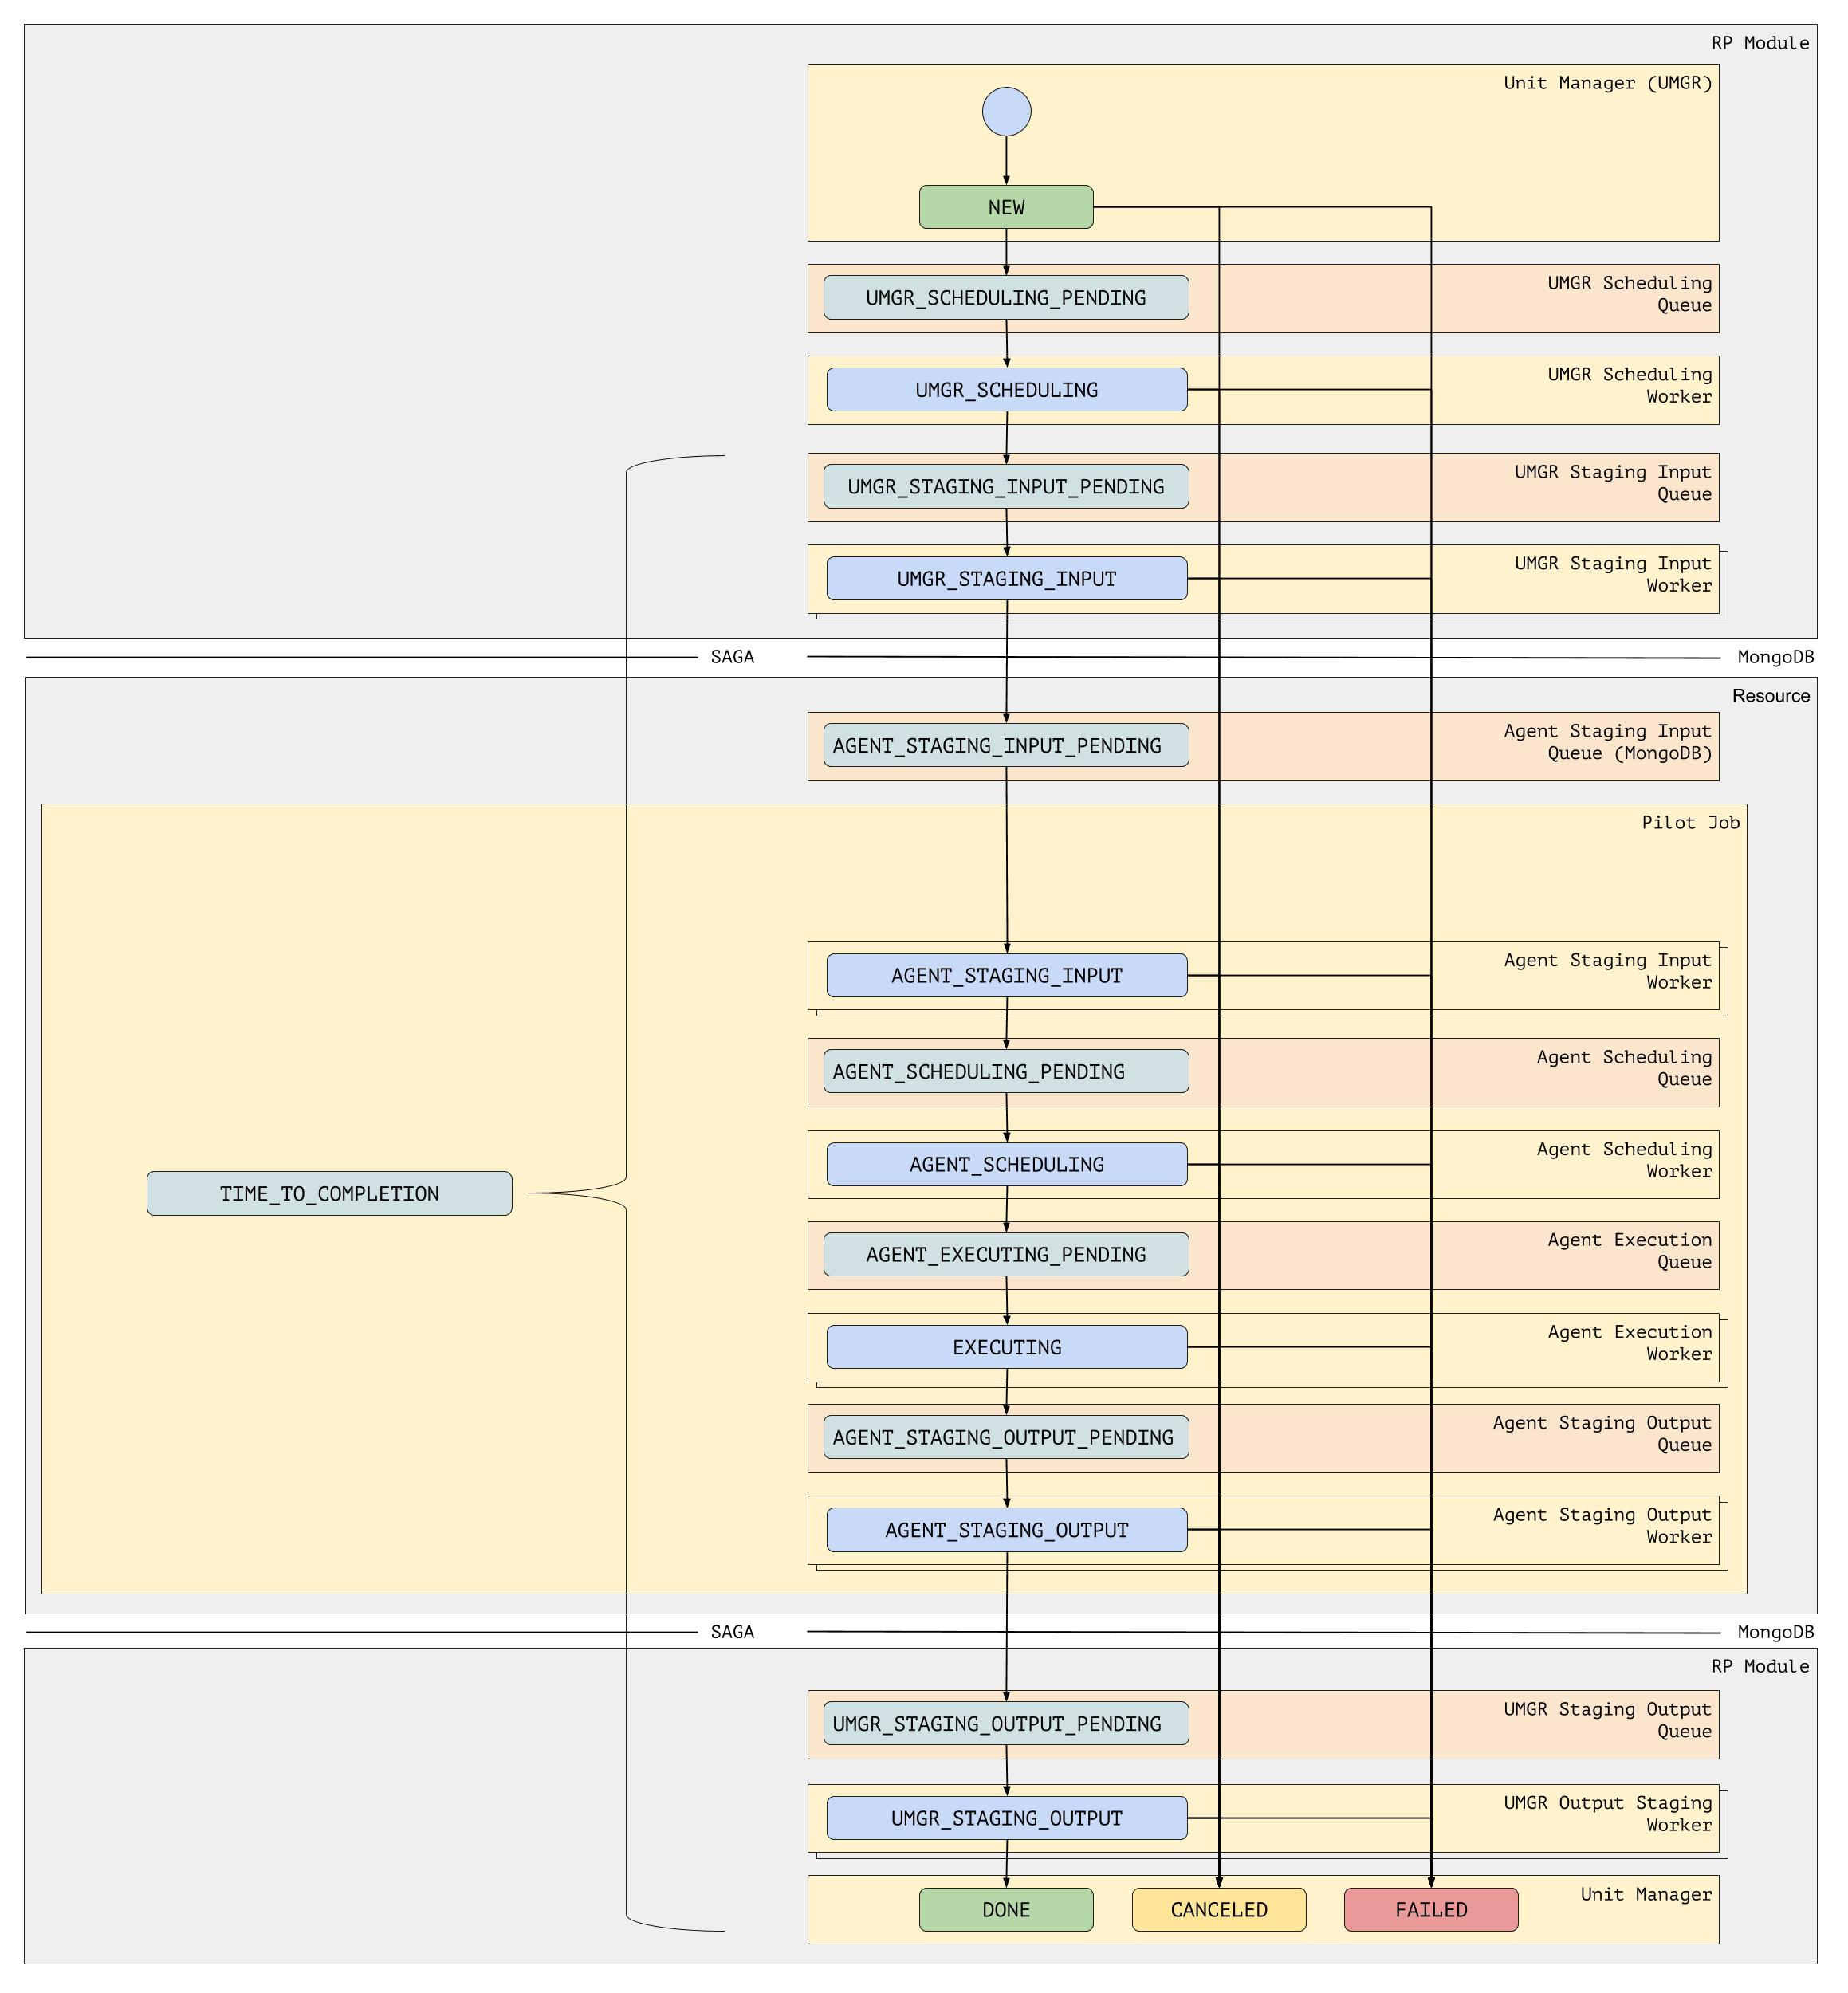
\includegraphics[width = 12cm, height = 12cm]{rp_state_model_mapping.jpg}
				\caption{Mapping of parameters to pilot state model. Derived from \cite{rp_state_diagram}.}
				\label{fig:pilot_state_mapping}
			\end{figure}

			As shown in Figure 2, the time-to-completion encompasses almost all of the states that the Pilot transitions through. This includes the staging of input for the Unit Manager and Agent, scheduling and executing simulations, and then staging the resultant data out to the Agent and Unit Manager. Formally, we state the time-to-completion in Equation 12:

			% Measurement equation
			\begin{align*}
				Time\_to\_Completion = DONE - UMGR\_STAGING\_INPUT\_PENDING \numberthis \label{12}
			\end{align*}

			This measurement, taken in seconds, provides us with the time necessary to complete a user's tasks.

		% Graphs and Analysis
		\subsubsection{Analysis}

			For each configuration of points and clusters, we graphed the time-to-completion across all cores.

			\begin{figure}[H]
				\centering
				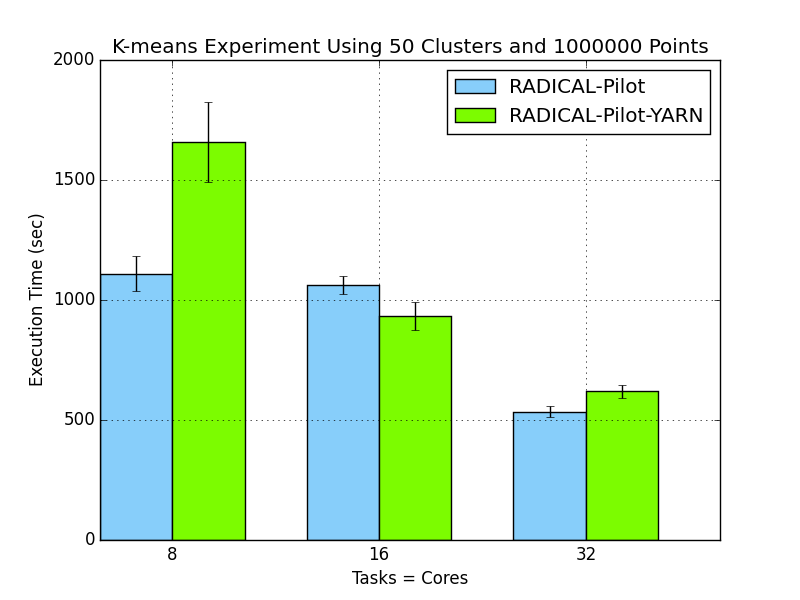
\includegraphics[scale=.50]{50.png}
				\caption{50 clusters, 1,000,000 points}
				\label{fig:50}
			\end{figure}

			In the configuration with 50 clusters, the first trend that we noticed is that the time-to-completion decreases as the core count increases. This is expected, since holding the total amount of computation the same and increasing the core count classifies this experiment as an instance of strong scaling. We observe this for both softwares. However, the comparisons between RADICAL-Pilot and RADICAL-Pilot-YARN do not yield a consistent pattern of increased performance in favor of RADICAL-Pilot-YARN. In the case with 8 cores, the time-to-completion for RADICAL-Pilot-YARN far outstrips that of RADICAL-Pilot, which is counter to the design goals RP-YARN. Scaling up to 16 cores, we notice that the relationship between the two softwares is reversed. RP time-to-completion exceeds that of RP-YARN in a range of about 20-200 seconds, within error bars. The comparison is decidedly in favor of RP-YARN, since it's time-to-completion is lower. In the case with 32 cores, the relationship reverts back to being in favor of RP. Yet, contrast in the execution times is much less than it was in the first case, indicating a difference of at most 200 seconds.

			\begin{figure}[H]
				\centering
				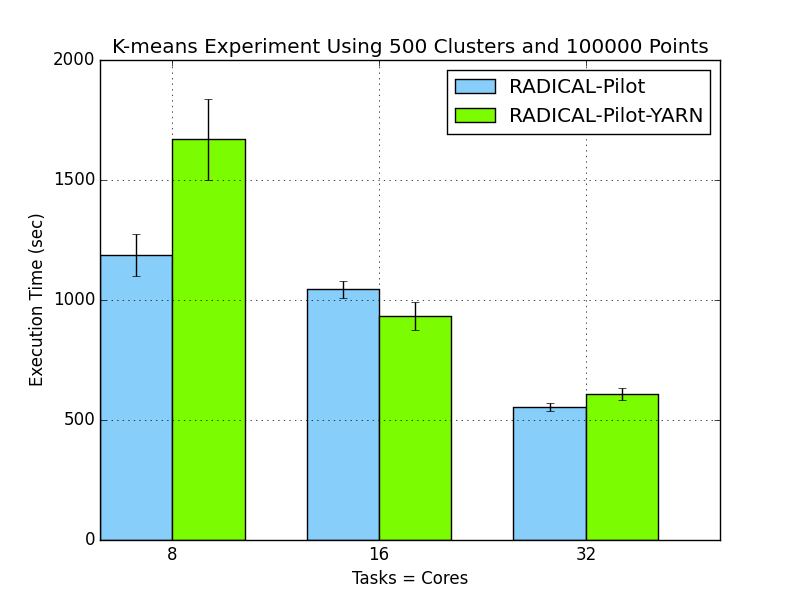
\includegraphics[scale=.50]{500.png}
				\caption{500 clusters, 100,000 points}
				\label{fig:500}
			\end{figure}

			Figure \ref{fig:500} shows the scaling behavior for the 500 cluster, 100,000 point case. The plots for the 500 and 50 cluster cases are remarkably similar. The 8 core case showed an increase in execution time for both RP and RP-YARN in comparison to the 50 cluster, 8 core case, but otherwise showed a similar disparity of time between the two softwares. RP execution time decreased slightly between the configurations for the 16 core case, but error bars indicate that RP statistically still takes longer than RP-YARN to run. Finally, the 32 core case shows a decrease in execution time for RP but an increase for RP-YARN, accentuating the relationship observed in the 50 cluster configuration. In summary, while there were fluctations in the times-to-completion of each execution, this configuration of cluster and points reinforced the trends noticed in the 50 cluster case. 

			\begin{figure}[H]
				\centering
				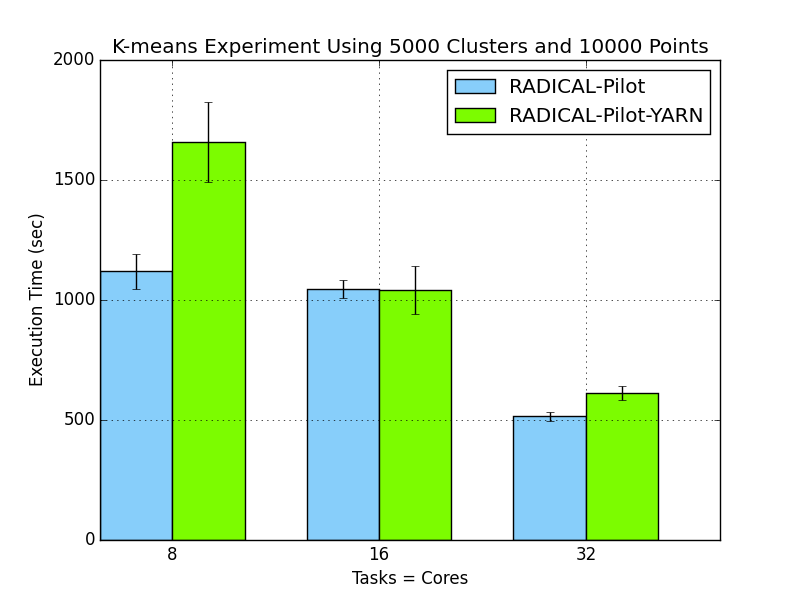
\includegraphics[scale=.50]{5000.png}
				\caption{5000 clusters, 10,000 points}
				\label{fig:5000}
			\end{figure}

			The 5000 cluster case also showed similarities to the trends in the 50 cluster and 500 cluster cases, as shown in Figure \ref{fig:5000}. Again, we see a large disparity in the execution times of RP and RP-YARN at 8 cores, ranging from 300 seconds to 700 seconds. The ratio between the two times relatively constant when compared to the 50 and 500 cluster cases. At 16 cores, we notice that the times-to-completion are almost identical, but the error bars give us more insight into the behavior. Since the error bar for RP-YARN is larger than that of RP, it is possible that the time-to-completion for RP-YARN may fluctuate between being greater than, less than, and equal to the time-to-completion for RP. At 32 cores, we see the largest difference of the three configurations between RP-YARN and RP, with a range of at most 200 seconds. Again, this supports the trends found in the other two cases. 

	\subsection{Reproducibility}
		The experiments described in this paper can be reproduced easily. All code for this work is located at the following links:
		\begin{enumerate}
			\item EnsembleMD: \url{https://github.com/Nikhil-Shenoy/RADICAL-research/tree/master/testing/summary}. 
			\item RADICAL-Pilot-YARN: \url{https://github.com/Nikhil-Shenoy/RADICAL-research/tree/master/yarn_replication/output_data}
		\end{enumerate}

		We enumerate the steps common to both experiments as follows:
		\begin{enumerate}
			\item Set up virtual environment on local machine using \url{virtualenv} tool.
			\item Acquire an account on the remote target machine. In this case, the target machine was XSEDE's Stampede.
			\item Generate a free MongoDB instance using MongoLab (\url{https://mlab.com/}) and note its access URL.	
			\item Once the experiment is ready to be run, use Tmux or another terminal multiplexer to start the job on your machine. You can detach from Tmux once the job begins executing on the remote target machine. It is recommended to start the job at night, as it will be completed by the next morning.
			\item If any errors occur while testing, remember to safely close and stop the Escript. Also make sure that the requrested resources are not still associated with one's account on the remote machine. One can verify this by logging in to that machine and checking the job status.
		\end{enumerate}

		Steps specific to EnsembleMD experiments:
		\begin{enumerate}
			\item Install the EnsembleMD Toolkit using the instructions found in the documentation at: \\
				  \url{http://radicalensemblemd.readthedocs.org/en/stable/installation.html}
			\item Modify the \url{bag_of_tasks.py} and the \url{simulation_analysis_loop.py} examples in the \url{radical.ensemblemd/examples} folder. This includes changing the kernels to Makefile and CharacterCount and changing the size of the input file to 10Mb
			\item For each core count in the scale [1,16,32,64,128], run the application at least four times. This allows the experimenter to verify the accuracy of his results.
			\item Set the resource to the remote target machine for which you now have an account.
			\item In the case of weak scaling, set the number of instances equal to the core count. In the case of strong scaling, set the number of instances to 1, but continue to alter the core count in the same way as in the weak scaling case.
			\item Remember to run all jobs with the following environment variables:
				\begin{itemize}
					\item RADICAL\_ENMD\_VERBOSE=DEBUG
					\item RADCIAL\_ENMD\_PROFILING=1
					\item RADICAL\_PILOT\_DBURL= <your mongodb url>
				\end{itemize}
		\end{enumerate}

		Steps specific to RADICAL-Pilot-YARN experiments:
		\begin{enumerate}
			\item Install RADICAL-Pilot using the instructions found in the documentation at: \\
			  \url{https://radicalpilot.readthedocs.io/en/stable/installation.html}
			\item No modifications to any of the Python files is required, unless there are problems with loading modules. If this is the case, then one should modify the instructions in the \url{pre_exec} phase of the Compute Unit to clear all modules and then reload the required modules.
			\item Once all modifications are made, the application can be started by passing the appropriate arguments to the \url{k-means.py} script. The parameters (in this order) are:
			\begin{itemize}
				\item Number of clusters
				\item Number of elements in each vector data point
				\item Number of cores to be used
				\item Number of tasks to be run
				\item Input data file
				\item Name of the output profile
				\item Name of scheduling queue
				\item Name of remote machine
			\end{itemize}
			\item To run all the configurations test for this paper, simply run the \url{run_yarn.py} script. This file cycles through and runs all of the 18 configurations displayed in the plots without requiring any additional parameters.
			\item All jobs require the following environment variables:
			\begin{itemize}
				\item RADICAL\_PILOT\_VERBOSE=DEBUG
				\item RADICAL\_PILOT\_DBURL= <your mongodb url>
			\end{itemize}
		\end{enumerate}

\section{Conclusion}
	This set of experiments were conducted to further understand the EnsembleMD Toolkit's scaling behavior. Based on the data from our experiments, we were able to identify trends that hinted at the Toolkit's capabilities for different core-task configurations. We considered stages of operation within the Toolkit that best exemplified its functionality; the Core Overhead, the Pattern Overhead, the RADICAL-Pilot Overhead, the Task Execution Time, and the Data Movement. While not all of these parameters showed distinct trends, we were able to glean information from a few of the parameters.

	The Task Execution time, for both the Makefile and Character Count steps, were found to be relatively constant across most configurations. This behavior is expected, as the time required to execute a bash shell command should only change if different input is given to it. In our case, the kernels in each step are doing the exact same tasks in every configuration, so a change in the execution time would be troubling. Even though the execution time was constant, we noticed that it was much higher than the time the same tasks took when executed from the Bash command prompt. This indicates that there are additional RADICAL-Pilot and EnsembleMD wrappings around the Bash commands that increase the duration. While dissecting that overhead was not the goal of this experiment, it is a candidate for future work.
	Throughout all the experiments performed, we observed that the EnsembleMD Core Overhead stayed relatively constant over all configurations. This implies that users and developers can rely on the performance of the EnMD Core staying constant regardless of the tasks the user gives it.
	
	In almost all measurements of the EnMD Pattern Overhead, we found that its duration was on the order of milliseconds. This is useful to users because they can be assured that any preparation done by EnMD to before executing the task is very efficient and is not expected to hinder the completion of the task. For developers, this indicates that the Toolkit makes quick transitions between states in the flow of execution.
	RP Overhead seems to scale in some cases, stay constant in other cases, and fluctuate in others. Because of this, we cannot extract a useful pattern and characterize RP's behavior at scale solely based on these experiments. As a majority of RP was implemented before EnMD, we would expect its performance at scale to have been worked on extensively and made reliable. We would need more experiments to properly pin down the behavior, as knowledge of how efficiently the pilot functions is crucial to the application's execution.

    In these experiments, we measured data movement as the time needed to download the output of our tasks from the remote machine to the local machine, seeing as all the input data was being generated on the remote machine. Both of the weak scaling cases showed that the time required for the data movement was directly proportional to the core/instance configuration. The Pipeline case seemed to imply a linear relationship between the variables, whlie the Simulation-Analysis case implied a more quadratic relationship. We have not investigated the relationship in detail, but determining such relationships would allow the user to restructure his application and explore the tradeoffs between effiency and data usage. Unfortunately, we were not able to notice distinct patterns in the strong scaling cases. We do believe that relationships similar to the ones suggested by the weak scaling experiments do exist, but further testing would be required to find them.

    The RADICAL-Pilot-YARN experiments were conducted to attempt to verify the performance benefits of the YARN extension to RADICAL-Pilot over the RADICAL-Pilot module by itself. We measured the time-to-completion of the different configurations of k-Means clustering as a way to simulate a user's experience with both softwares and tried to empirically demonstrate the capabilities of the new extensions. While the theory and design decisions behind RADICAL-Pilot-YARN are sound, the evidence that we found through our experiments currently does not support it. On the other hand, the data does not decisively reject the expectation that RADICAL-Pilot-YARN should incur a smaller time-to-completion. Across the three configurations of clusters and points, we observe that, in the cases of 8 and 32 cores, that RP-YARN always had a larger time-to-completion than that of RP by itself. However, the ratio between the execution time for RP-YARN and RP at 8 cores is larger than it is at 32 cores. This may imply that the two softwares have similar performance at high core counts, and that a difference in performance can only be noticed at lower core counts. A possible reason for this may be that an increased overhead incurred by the YARN components at lower core counts, but that penalty becomes reduced as more cores are added. The other significant trend across all configurations was that of the 16 core cases; in two out of the three, RADICAL-Pilot was observed to have a larger time-to-completion than RADICAL-Pilot-YARN. In the third case, the times-to-completion were essentially equal in mean value, but the error bars demonstrated that the RP-YARN time could fluctuate from being greater than RP to less than RP. Two immediate implications can arise out of this; if, in subsequent experiments, RP-YARN is shown to have a greater time-to-completion than RP, then the result would aid in rejecting the theory behind adding the YARN components to RADICAL-Pilot. All but two configurations of cluster, points, and cores would show that RP-YARN is outpaced by RP, suggesting that the YARN components are not necessary. Alternatively, the RP-YARN time being less than the RP time would only lead to additional inconclusive evidence, as no clear relationship between RP and RP-YARN can be established. In summary, these experiments have not been able to successfully verify the advantage of adding the YARN scheduling and resource management components to the existing RADICAL-Pilot software. The evidence seemingly indicates that RADICAL-Pilot-YARN actually slows down the performance of the system, arguing against the theoritcal underpinnings of the YARN extensions.

\section{Future Work}
	Performance testing is an ongoing body of work in any scientific experiment, and the results presented here can be extended into any different directions. First, one could examine the relationship between the time taken to process varying sizes of data and the number of cores given to process that data. Such information would be useful in gauging EnsembleMD`s capability to handle large and small amounts of data. The same experiments could be run on all the high performance machines supported by the Toolkit, with the expectation that the user gets similar performance no matter which machine he uses. Next, one could consider the Toolkit`s role in data movement; in these experiments, we considered only the Toolkit`s involvement in transfers between the local and remote machine. An interesting avenue to explore would be the duration of all the operations and changes that the Toolkit makes to the data while it is on the remote node but not being processed. This, combined with this article`s measurment of local/remote transfers, may better reflect the overhead incurred by data movement. Finally, discovery of best-fit functions for the important components of the Toolkit, such as the Pattern Overhead, RP Overhead, and Data Movement, would characterize the Toolkit in an easy-to-use way. The benefit of using a simple function to approximate the behavior of a Toolkit component would provide the user with instant information on how to structure his application, leading to increased usability.

	The RADICAL-Pilot-YARN experiments can and should be extended to analyze the full relationship between RADICAL-Pilot and RADICAL-Pilot-YARN. Verification of our experimental results would be useful to those currently developing additional YARN functionality for RADICAL-Pilot, as the performance information can suggest whether the new modules are necessary. Additional work can explore the relationship between cores and each configuration by utilizing higher core counts, machine permitting. Such an experiment would verify whether the performance of RADICAL-Pilot and RADICAL-Pilot-YARN becomes indistinguishable at larger core counts. Finally, one could perform a formal comparison between the results obtained in \cite{hadoop_paper} and our results to find out the changes made to RADICAL-Pilot in the intervening time. The additions in the six-month time period could provide insight into the behavior RADICAL-Pilot in these experiments.

\section{Lessons Learned}
	Analyzing the performance of a system can lead to many insights about the system, and about the attitude with which one approaches experimentation in general. During our experience with testing the EnsembleMD Toolkit, RADICAL-Pilot, and RADICAL-Pilot-YARN, we learned a variety of concepts which we believe have improved our abilities as researchers.

	One of the most important concepts we learned about is careful design of experiments. At the beginning of our experimentation, we had a tendency to dive into the data head first without a solid plan for what we were measuring. We tried to find relationships between every pair of variables in the data set, but soon learned that this was much too inefficient to produce good results. In many of those tests, the relations we found did not yield any useful information about the system, which rendered all the time spent running those simulations useless. Not only would these types of experiments not produce results, but adding just one variable would dramatically increase the complexity of running the entire set of simulations. After this experiment, we learned to focus on specific behaviors of the system we wanted to examine, such as strong scaling, and tailored our experiments towards those. This resulted in concise, informative results that provided useful information for the development team.

	We also understood the importance of reproducibility of experiments. Providing the parameters to reproduce an experiment allows us to go back to the experiment after some time and still expect to have the same results. Also, others can look at our work, run the same experiment, and verify whether our interpretation of the data is valid. In the greater scientific community, reproducibility allows a scientist to test the foundations on which his current experiment is based. If he thinks his experiment went wrong based on work done by others, he can go and re-run the experiment to either verify or change his assumptions. Sometimes the initial interpretation of the results was wrong, and another trial yielded a more significant, appropriate result. This allows the community to make sure that the assumptions from previous experiments are a solid foundation upon which new work can be done.

	Adapting existing code to our experiments improved our skills as developers and widened our knowledge of the softwares we used and the rest of the RADICAL Cybertools stack. In the all the projects we had done before joining the group, we were required to implement all functionality from scratch, which augmented my understanding of class concepts but did not reflect real software development. In designing the experiments, we were forced to look at code written by others, understand it, and adapt it to our work. As we read, we understood why layers of abstraction were implemented between components of each software, and between layers of the RADICAL Cybertools stack. Our view of the system changed from a collection of disjoint Pilot operations into a series of well-defined state transitions. Learning about the architecture in this way gave our experiments more context, and allowed us to remove measurements which didn't capture the interactions between important components. 

	Finally, we gained a greater appreciation for reading technical papers. After we read a variety of papers written by RADICAL developers and other members of the community, we understood that impactful papers require careful design in order to be useful. In specific, the specific sections of a paper must have a clear focus and a proper transition into the following section. We especially noticed how important the introduction and background are in setting the context for the experiment. If carefully crafted, then the user will be more willing to read the rest of the paper and understand why one's work is so important. The sections describing the experiment must be detailed, yet concise. It is best to include only enough information to reproduce the experiment and explain why the work is being done; any more information could cause the reader to become confused and lose sight of the experiment's purpose. Finally, the analysis and conclusion should bridge the context laid out in the opening sections and the results from the experiment to summarize the impact of the work. While many essays and other pieces of writing do a have a similar structure, we were able to learn how the scientific community adapted that structure to fit its needs and present its work to the world. Going forward, we can make use of this in order to make our own contributions.

% Using no_cite to make sure all the bib entries are processed
\nocite{pstar}
\nocite{saga_paper}
\nocite{rp_arch}
\nocite{k_means}
\nocite{apache_hadoop_yarn}
\nocite{hadoop_paper}

\bibliography{final_paper}{}
\bibliographystyle{IEEEtran}		
\end{document}